\date{}
\title{}
\date{}
\usepackage[outputdir=latex.out]{minted}
\begin{document}
\begin{frame}
    \titlepage
\end{frame}


\makeatletter
\newenvironment<>{btHighlight}[1][]
{\begin{onlyenv}#2\begingroup\tikzset{bt@Highlight@par/.style={#1}}\begin{lrbox}{\@tempboxa}}
{\end{lrbox}\bt@HL@box[bt@Highlight@par]{\@tempboxa}\endgroup\end{onlyenv}}

\newcommand<>\btHL[1][]{%
  \only#2{\begin{btHighlight}[#1]\bgroup\aftergroup\bt@HL@endenv}%
}
\def\bt@HL@endenv{%
  \end{btHighlight}%   
  \egroup %
}
\tikzset{
    btHLbox/.style={
        fill=red!30,outer sep=0pt,inner xsep=1pt, inner ysep=0pt, rounded corners=3pt
    },
}
\newcommand{\bt@HL@box}[2][]{%
  \tikz[#1]{%
    \pgfpathrectangle{\pgfpoint{1pt}{0pt}}{\pgfpoint{\wd #2}{\ht #2}}%
    \pgfusepath{use as bounding box}%
    \node[text width={},draw=none,anchor=base west, btHLbox, minimum height=\ht\strutbox+1pt,#1]{\raisebox{1pt}{\strut}\strut\usebox{#2}};
  }%
}

\lst@CCPutMacro
    \lst@ProcessOther {"2A}{%
      \lst@ttfamily 
         {\raisebox{2pt}{*}}% used with ttfamily
         {\raisebox{2pt}{*}}}% used with other fonts
    \@empty\z@\@empty

\lstdefinelanguage
   [x8664gas]{Assembler}     % add a "x64" dialect of Assembler
   [x86masm]{Assembler} % based on the "x86masm" dialect
   % with these extra keywords:
   {morekeywords={CDQE,CQO,CMPSQ,CMPXCHG16B,JRCXZ,LODSQ,MOVSXD,%
                  POPFQ,PUSHFQ,SCASQ,STOSQ,IRETQ,RDTSCP,SWAPGS,.TEXT,.STRING,.ASCIZ,%
                  BEQ,LW,SW,LB,SB,ADDIU,J,BEQZ,BNEZ,BNE,%
                  MOVUPD,MULPD,MOVSD,MULSD,%
                  SHLADD,MOV,CMP.LT,TBIT.NZ,BR.RET.SPTK.MANY,%
                  ADDQ,POPQ,PUSHQ,RRMOVQ,MRMOVQ,RMMOVQ,IRMOVQ,%
                  <-,LL,SC,ADDI,ADDL,VMOVDQA,ADDQ,CMPL,JB,JBE,MOVL,CLTQ,%
                  MOVW,PUSHW,MOV,ADD,SUB,INT,PUSH,MOV,ADD,REP,MOVSB,%
                  TESTQ,CMPQ,MOVL,MOVQ,ADDQ,JMPQ,XORQ,%
                  LEAQ,LEAL,LEA,RETQ,RET,POPL,POPW,PUSHL,PUSHW,%
                  LEAW,%
                  SUBQ,SYSCALL,.ASCII,CALLQ,MOVSLQ,JMP,ANDQ,SHRQ,MOVB,INCQ,TESTL,XORL,%
                  SHRL,LEAL,SARL,SUBL,IMULL,IMULQ,MOVDQU,PADDD,XORL,%
                  MOVZBL,MOVZB,SHRB,SRAL,SHRL,ANDL,%
                  CMOVNS,SRAL,SRAQ,MOVZBW,MOVZBQ,%
                  PADDW,PADDQ,MODUPS,MOVAPD,%
                  MOVL,RET,.GLOBL,%
		  PAUSE,LFENCE,JMP,%
                  },
    deletekeywords={eax,ebx,sp,si,cx,di,ds,cs,es,fs,dx,ax,bx,al,esi,ebp,ecx,rip,eip,edx,edi,rdi,esp},
    deletekeywords=[2]{size},
    alsoletter={\%},
    alsoother={()},
    emphstyle={\color{violet!50!black}},
    emph={\%rax,\%rbx,\%rcx,\%rdx,\%r8,\%r9,\%r10,\%r11,\%r12,\%r13,\%r14,\%r15,\%eax,\%ebx,\%sp,\%si,\%cx,\%di,\%ds,\%cs,\%es,\%fs,\%dx,\%ax,\%bx,\%al,\%esi,\%ebp,\%ecx,\%rip,\%eip,\%edx,\%edi,\%rdi,\%esp,\%rsp},
    %moreemph={eax,ebx,sp,si,cx,di,ds,cs,es,fs,dx,ax,bx,al,esi,ebp,ecx,rip,eip,edx,edi,rdi,esp},
    morecomment=[l]{\#},
    morecomment=[l]{\/\/},
    morecomment=[s]{/*}{*/},
    sensitive=false,
    keepspaces=true} % et

\lstalias[]{myasm}[x8664gas]{Assembler}

\lstdefinelanguage{JavaScript}{
  keywords={typeof, new, true, false, catch, function, return, null, catch, switch, var, if, in, while, do, else, case, break},
  ndkeywords={class, export, boolean, throw, implements, import, this},
  sensitive=false,
  comment=[l]{//},
  morecomment=[s]{/*}{*/},
  morestring=[b]',
  morestring=[b]"
}

\newcommand{\keywordstyle}{\sourcecodeprolight\bfseries\color{blue!30!black}}
\newcommand{\stringstyle}{\color{blue!20!black}\ttfamily}

\lstset{
    language=C,
    basicstyle=\sourcecodepro\EmptyMapping,
    escapechar=`,
    keywordstyle=\keywordstyle\EmptyMapping,
    identifierstyle=\sourcecodepro\EmptyMapping,
    numberstyle=\small\color{black!70},
    commentstyle=\color{red!60!black}\ttfamily\itshape,
    stringstyle=\color{blue!20!black}\ttfamily,
    ndkeywordstyle=\bfseries\color{blue!30!black},
    upquote=true,
}



\lstdefinestyle{medium}{
    basicstyle=\sourcecodepro\EmptyMapping\fontsize{12}{13}\selectfont,
    keywordstyle=\sourcecodepro\EmptyMapping\fontsize{12}{13}\selectfont\keywordstyle,
}

\lstdefinestyle{small}{
    basicstyle=\sourcecodepro\EmptyMapping\small,
    keywordstyle=\sourcecodepro\EmptyMapping\small\keywordstyle,
}

\lstdefinestyle{smaller}{
    basicstyle=\sourcecodepro\EmptyMapping\fontsize{11}{12}\selectfont,
    keywordstyle=\sourcecodepro\EmptyMapping\fontsize{11}{12}\selectfont\keywordstyle,
}

\lstdefinestyle{size105}{
    basicstyle=\sourcecodepro\EmptyMapping\fontsize{10.5}{11.5}\selectfont,
    keywordstyle=\sourcecodepro\EmptyMapping\fontsize{10.5}{11.5}\selectfont\keywordstyle,
}

\lstdefinestyle{size10}{
    basicstyle=\sourcecodepro\EmptyMapping\fontsize{10}{11}\selectfont,
    keywordstyle=\sourcecodepro\EmptyMapping\fontsize{10}{11}\selectfont\keywordstyle,
}

\lstdefinestyle{size9}{
    basicstyle=\sourcecodepro\EmptyMapping\fontsize{9}{10}\selectfont,
    keywordstyle=\sourcecodepro\EmptyMapping\fontsize{9}{10}\selectfont\keywordstyle,
}
\lstdefinestyle{size8}{
    basicstyle=\sourcecodepro\EmptyMapping\fontsize{8}{9}\selectfont,
    keywordstyle=\sourcecodepro\EmptyMapping\fontsize{8}{9}\selectfont\keywordstyle,
}



\lstdefinestyle{script}{
    basicstyle=\sourcecodepro\EmptyMapping\scriptsize,
    keywordstyle=\sourcecodepro\EmptyMapping\scriptsize\bfseries,
}




\begin{frame}{last time}
    \begin{itemize}
    \item challenges with system call filtering
    \vspace{.5cm}
    \item privilege separation idea
    \item limits on what it does/does not mitigate
    \vspace{.5cm}
    \item started: idea of choosing what program can name
    \end{itemize}
\end{frame}

\begin{frame}{some FUZZ notes}
    \begin{itemize}
    \item fuzz program suddenly stops --- memory limit probably too low
    \item if number of tests per unit time is low
        \begin{itemize}
        \item make base inputs simpler
        \item worried about something not being in starting inputs? make multiple base cases
        \end{itemize}
    \end{itemize}
\end{frame}

\begin{frame}{assignment Q+A}
\end{frame}

\subsection{versus capability-type approach}
\begin{frame}{changing what programs can name}
    \begin{itemize}
    \item seccomp, separate users: program tries to access X, checks if allowed
    \vspace{.5cm}
    \item alternate idea: changing what Xs program can name
    \end{itemize}
\end{frame}

\begin{frame}{aside: capabilities/ambient authority (1)}
    \begin{itemize}
    \item user permissions --- authority tied to each running program
    \item ``access control lists'' for resources
    \item sometimes called ``ambient authority''
    \vspace{.5cm}
    \item alternate model: ``capabilities''
    \item running program has list of things it can access/how
    \end{itemize}
\end{frame}

\begin{frame}{aside: capabilities/ambient authority (2)}
    \begin{itemize}
    \item capabilities = program has list of things it can access
    \item most common thing with design: open files
    \vspace{.5cm}
    \item used as basis of some operating system designs
        \begin{itemize}
        \item not desktop OSes, but\ldots
        \item Unix/Linux has many things with `flavor' of capabilities
        \end{itemize}
    \item in ``fully'' capability-based OSes also\ldots
        \begin{itemize}
        \item capabilities for accessing non-regular-file resources (processes, directories,
            network ports, \ldots)
        \item way of transferring capabilities between programs (instead of, e.g., filenames/PIDs/etc.)
        \item OS doesn't track user IDs/etc. (though maybe system services do)
        \end{itemize}
    \end{itemize}
\end{frame}


\subsection{chroot}
\begin{frame}{Unix filesystems and mounting}
    \begin{itemize}
    \item my Linux desktop has two disks:
        \begin{itemize}
        \item \texttt{/} --- an SSD
        \item \texttt{/mnt/extradisk} --- a hard drive
        \end{itemize}
    \item hard drive appears as \textit{subdirectory} of SSD
    \item subdirectory called a \textit{mount point}
    \end{itemize}
\end{frame}

\begin{frame}[fragile,label=perProcessRoot]{per-process root}
    \begin{itemize}
    \item on Unix: each process tracks its own root directory (/)
    \item can be changed with chroot() system call
        \begin{itemize}
        \item command-line tool to access: \texttt{chroot}
        \end{itemize}
    \vspace{.5cm}
    \item usage: can isolate program from other files on system
        \begin{itemize}
        \item example: limit what public file server can access?
        \end{itemize}
    \end{itemize}
\end{frame}

\begin{frame}[fragile,label=lsChrootExample]{chroot ls}
\begin{lstlisting}[language={},style=smaller]
# mkdir /tmp/example
# cp /bin/ls /tmp/example/ls
# chroot /tmp/example /ls
chroot: failed to run command ‘/ls’: No such file or directory
# cp -r /lib64 /tmp/example/lib64
# mkdir -p /tmp/example/lib
# cp -r /lib/x86_64-linux-gnu /tmp/example/lib/x86_64-linux-gnu
# chroot /tmp/example /ls
/ls: error while loading shared libraries: libpcre2-8.so.0: cannot open shared object file: No such file or directory
# cp /usr/lib/x86_64-linux-gnu/libpcre2-8* /tmp/example/lib/x86_64-linux-gnu
# chroot /tmp/example /ls /
lib  lib64  ls
# chroot /tmp/example /ls /..
lib  lib64  ls
# 
\end{lstlisting}
\end{frame}

\begin{frame}{chroot escapes}
    \begin{itemize}
    \item chroot prevents accessing files outside the new \texttt{/}
    \item but root (system adminstrator) user in chroot can access disks, etc.
    \vspace{.5cm}
    \item typical usage: combine chroot with extra user
    \end{itemize}
\end{frame}

\begin{frame}{chroot impracticality}
    \begin{itemize}
    \item some things make chroot impractical in general:
    \vspace{.5cm}
    \item seems like one needs extra copies of most of the system
    \item hard to communicate between separate roots
    \item requires administrator permissions to configure
        \begin{itemize}
        \item dangerous to let normal users configure b/c they could confuse priviliged (set-user-ID) programs like \texttt{sudo}
        \end{itemize}
    \end{itemize}
\end{frame}


\subsubsection{exercise}
\begin{frame}{exercise}
    \begin{itemize}
    \item what scenarios does chroot make most/least sense for?
    \begin{itemize}
        \item A. the rendering part of web browser
        \item B. a web server
        \item C. a media player
        \item D. a network time server (for other machines to set their clocks)
    \end{itemize}
    \end{itemize}
\end{frame}


\subsection{Linux namespaces}
\begin{frame}{Linux namespaces (1)}
    \begin{itemize}
    \item Linux: alternate sandboxing features
    \item ``namespaces'' for other resources
    \item chroot: each process has own idea of root directory
        \begin{itemize}
        \item change to OS: look up root directory in process, not global variable
        \end{itemize}
    \item can apply this to other resources:
        \begin{itemize}
        \item what filesystems (disks) are available
        \item what network devices are available
        \item what user identifier numbers are
        \item \ldots
        \end{itemize}
    \end{itemize}
\end{frame}

\begin{frame}{Linux namespaces (2)}
    \begin{itemize}
    \item user namespace:
    \vspace{.5cm}
    \item can run programs with new view of users:
    \vspace{.5cm}
    \item inside namespace: running as root
    \item outside namespace: root translated to innocent user ID
    \item allows running programs that expect different users
        \begin{itemize}
        \item \ldots without changes, but without giving special permissions
        \end{itemize}
    \vspace{.5cm}
    \item mechanism: reassign user ID numbers in kernel
        \begin{itemize}
        \item figuring out what user ID means --- always apply current process mapping
        \end{itemize}
    \end{itemize}
\end{frame}

\begin{frame}[fragile,label=LinuxCloneUnshare]{aside: Linux clone(), unshare() syscalls}
\begin{itemize}
\item Linux clone system call: start new process (or thread)
\item flags to specify environment of new process
\item these flags can include ``make a new namespace of a type''
\end{itemize}
\begin{lstlisting}[style=smaller,language=C++]
int id = clone(start_function, ..., CLONE_NEWUSER | other-flags);
\end{lstlisting}
\begin{itemize}
\item above option: new user namespace for new process
\vspace{.5cm}
\item alternative: for changing current process's namespace:
\end{itemize}
\begin{lstlisting}[style=smaller,language=C++]
unshare(CLONE_NEWUSER);
\end{lstlisting}
\end{frame}

\begin{frame}{user namespaces API}
\begin{itemize}
\item Linux: users identified by numerical \textit{user IDs} (UIDs)
\vspace{.5cm}
\item with user namespaces:
\item control file \texttt{/proc/PROCESS-ID/UID\_MAP} contains lines like:
    \begin{itemize}
    \item \texttt{0 1000 2} --- UID 0--1 maps to UID 1000--1001
    \item \texttt{1000 2000 100} --- UID 1000-1100 maps to UID 2000--2100
    \end{itemize}
\item can write to that file to reconfigure (if enough permissions)
\end{itemize}
\end{frame}

\begin{frame}{Linux namesapces (3)}
    \begin{itemize}
    \item mount namespaces:
        \begin{itemize}
        \item Unix: mounting disk = making the contents of the disk available as directories+files
        \end{itemize}
    \vspace{.5cm}
    \item different idea of what filesystems are available
    \item can be setup with \textit{bind mounts} to ``real FS''
        \begin{itemize}
        \item but otherwise: no access to directories outside mount namespace
        \item normally requires root --- but special case with user namespaces
        \end{itemize}
    \end{itemize}
\end{frame}

\begin{frame}[fragile,label=mountNSCmdLine]{mount namespaces API}
from command line:
\begin{lstlisting}[language={},style=smaller]
    # runs shell (/bin/sh) in new mount namesapce
shell1$ unshare --mount /bin/sh

    # setup directories in /tmp/workdir and make them aliases of things on normal FS 
    # these aliases will only exist for processes in mount namespace
shell2$ mkdir -p /tmp/workdir/bin
shell2$ mkdir -p /tmp/workdir/lib
shell2$ mkdir -p /tmp/workdir/usr
shell2$ mkdir -p /tmp/workdir/current
shell2$ mount -o bind,ro /bin /tmp/workdir/bin
shell2$ mount -o bind,ro /lib /tmp/workdir/lib
shell2$ mount -o bind,ro /usr /tmp/workdir/usr
shell2$ mount -o bind /home/someuser /tmp/workdir/current

    # start new shell with the root directory being /tmp/workdir
shell2$ chroot /tmp/workdir /bin/sh
shell3$ cd /
shell3$ /bin/ls
bin     current     lib     usr
\end{lstlisting}
\end{frame}

\begin{frame}{Linux namespaces (3)}
    \begin{itemize}
    \item user namespace and mount namespace together:
    \vspace{.5cm}
    \item run program in new user namespace
    \item map regular root (in namespace) to regular user
        \begin{itemize}
        \item ``opts out'' of programs like sudo
        \end{itemize}
    \item move to new mount namespace
    \item setup bind mounts + chroot
        \begin{itemize}
        \item special case: allowed because root in user namespce
        \item can't get ``real'' root (administrator) privileges ever
        \end{itemize}
    \item run program with subset of available files
    \end{itemize}
\end{frame}

\begin{frame}{Linux namespaces (4)}
    \begin{itemize}
    \item other resources with namespaces
    \item network --- common usage: virtual network device for set processes
        \begin{itemize}
        \item different ``what is my IP address?'' answer for different processes
        \end{itemize}
    \item hostname (``UTS'')
    \item process identifiers
    \item control groups (resource limits for memory, CPU usage, disk I/O, etc.)
    \end{itemize}
\end{frame}

\begin{frame}{Linux control groups}
    \begin{itemize}
    \item control groups --- tied to namespaces
    \item primarily: CPU/memory/IO performance restrictions
        \begin{itemize}
        \item primarily intended for `friendly sharing' (containers, etc.)
        \item important for preventing denial-of-service/etc.
        \item not as big a security conern as file/user/etc. access
        \end{itemize}
    \item also mechanism for adding IO device restrictions
    \item also mechanism to start/stop a bunch of processes together
    \end{itemize}
\end{frame}


% FIXME: Chrome sandboxing failing:
    % https://theori.io/research/escaping-chrome-sandbox/
        % Binder (Chrome internal IPC library)
    % % https://googleprojectzero.blogspot.com/2020/04/you-wont-believe-what-this-one-line.html
    % https://bugs.chromium.org/p/project-zero/issues/detail?id=1991
    % https://bugs.chromium.org/p/project-zero/issues/detail?id=1985

% FIXME: SELinux sandbox escape:
    % https://www.openwall.com/lists/oss-security/2016/09/25/1

\subsection{Linux programs that attempt confinement}
\begin{frame}{Linux sandboxing programs, generally}
    \begin{itemize}
    \item docker, lxc, lxd, containerd
        \begin{itemize}
        \item use namespaces to create ``container'' with own copy of OS libraries, services
        \item but containers share OS `kernel' and potentially files with host unlike VM
        \item (might also have options to use other ways of getting this functionality --- VM's, etc.)
        \end{itemize}
    \item bubblewrap, firejail
        \begin{itemize}
        \item use Linux namespace tools + ``bind mounts'' to give programs only subset of files, etc.
        \item firejail has option of running a ``proxy'' windowing system server
        \end{itemize}
    \item SELinux's sandbox
        \begin{itemize}
        \item uses Security Enhanced Linux's mandatory access controls instead of Linux namespaces
        \item includes option for ``proxy'' for windoing system server
        \end{itemize}
    \end{itemize}
\end{frame}


\subsection{containers}
\begin{frame}{containers}
    \begin{itemize}
    \item Linux's seccomp + namespaces + SELinux commonly used to implement containers
        \begin{itemize}
        \item (plus cgroups (control groups) for performance isolation)
        \end{itemize}
    \vspace{.5cm}
    \item usual goal: looks like virtual machine, but much lower overhead
    \item examples: Docker, Kubernetes
        \begin{itemize}
        \item (note: these may also support other ways of creating `lightweight VMs')
        \end{itemize}
    \end{itemize}
\end{frame}





\subsubsection{runC bug}
\begin{frame}{runc bug}
    \begin{itemize}
    \item 2019 bug in Docker, other container implementations (CVE-2019-5736)
        \begin{itemize}
        \item blog post for vulnerability finders: \\\scriptsize \url{https://blog.dragonsector.pl/2019/02/cve-2019-5736-escape-from-docker-and.html}
        \end{itemize}
    \vspace{.5cm}
    \item bug setup:
        \begin{itemize}
        \item user starts malicious container X
        \item user tells docker to start a new command in malicious container X
        \item \myemph<2>{malicious container X hijacks the ``new command'' starting program}
        \item hijacked program used to access stuff outside container
        \end{itemize}
    \item part of problem: Docker and others weren't using user namespaces at the time
        \begin{itemize}
        \item compatability problems
        \end{itemize}
    \end{itemize}
\end{frame}

\begin{frame}{setup: /proc/PID}
    \begin{itemize}
    \item Linux provides /proc directory to access info about programs
    \item used for implementing process list utils, debugging
        \begin{itemize}
        \item needed to make a functional container
        \end{itemize}
    \item subdirectory for each process in current container
        \begin{itemize}
        \item process ID PID has /proc/PID subdirectory
        \item /proc/self is alias for current process's subdirectory
        \end{itemize}
    \vspace{.5cm}
    \item included is /proc/PID/exe file --- alias for executable file
    \end{itemize}
\end{frame}

\begin{frame}{running a command in existing container}
    \begin{itemize}
    \item to run command X in existing container:
    \vspace{.5cm}
    \item step 1: switch current process to that container
    \item<2-> \myemph{code in container can access /proc here?}
    \item<2-> \myemph{including overwriting /proc/self/exe!}
        \begin{itemize}
        \item which is a program run as root!
        \end{itemize}
    \vspace{.25cm}
    \item step 2: execute command X
    \end{itemize}
\end{frame}


\begin{frame}{partial fix}
    \begin{itemize}
    \item can disable access to /proc/PID/exe (and related things)
    \item system call: \texttt{prctl(PR\_SET\_DUMPABLE, 0)}
    \item but\ldots the run-in-container tool did this for a while
    \vspace{.5cm}
    \item<2-> problem: this gets reset on executing a new program
    \item<2-> and attacker could make the new program be /proc/PID/exe
        \begin{itemize}
        \item one mechanism: symbolic links (file aliases)
        \end{itemize}
    \item<2-> but change dynamic linking setup to run attacker code
    \item<2-> \ldots which accesses /proc/self/exe
    \end{itemize}
\end{frame}

\begin{frame}{full fix}
    \begin{itemize}
    \item make single-use copy of start-in-container tool each time command run
        \begin{itemize}
        \item in-memory file
        \end{itemize}
    \item \ldots so modifying it doesn't change anything
        \begin{itemize}
        \item (but it's also protected from modification)
        \end{itemize}
    \vspace{.5cm}
    \item other solutions:
        \begin{itemize}
        \item make executable non-writable (e.g. SELinux, don't run container as root)
        \end{itemize}
    \end{itemize}
\end{frame}


\subsubsection{Chrome sandbox escapes}
\begin{frame}{Chrome sandbox escape (1)}
    \begin{itemize}
    \item recall: renderer communicates with `browser kernel'
    \item `browser kernel' might have bugs in this interface
        \begin{itemize}
        \item example: \url{https://project-zero.issues.chromium.org/issues/42451090} --- missing access check for `wrong' website
        \item example: \url{https://chromereleases.googleblog.com/2021/09/stable-channel-update-for-desktop.html} \url{https://starlabs.sg/blog/2022/01-the-cat-escaped-from-the-chrome-sandbox/} --- use after free in API available from renderer
        \end{itemize}
    \end{itemize}
\end{frame}

\begin{frame}{Chrome sandbox escape (2)}
    \begin{itemize}
    \item Chrome Windows sandbox
    \item based on ``restricted access tokens''
        \begin{itemize}
        \item on Windows, programs have `access tokens' representing their permissions
        \item can create `restricted' version to limit access
        \end{itemize}
    \end{itemize}
\end{frame}
\begin{frame}{Chrome sandbox escape (3)}
    \begin{itemize}
    \item {\tiny \url{https://googleprojectzero.blogspot.com/2020/04/you-wont-believe-what-this-one-line.html}}:
    \item problem: Windows erronously allowed starting new processes with a more unrestricted token
        \begin{itemize}
        \item supposed to have check where the token being used came from, but incomplete
        \end{itemize}
    \item \ldots but needed to get `handle' to that token
    \item solution: ask to duplicate another running process
    \end{itemize}
\end{frame}



\section{the Android sandbox}
\begin{frame}{Android sandbox}
    \begin{itemize}
    \item Android --- Linux based OS for phones/tablets
    \vspace{.5cm}
    \item \url{https://source.android.com/security/app-sandbox}
    \item current version: SELinux + seccomp (system call filter)
    \end{itemize}
\end{frame}


% FIXME: Android sandbox

\subsection{OSX sandboxing}

\begin{frame}{OS X sandboxing}
    \begin{itemize}
    \item OS X (tries to) implement system call filtering
    \item main challenge: what about files?
        \begin{itemize}
        \item user can open a file anywhere --- we expect that to work
        \end{itemize}
    \item<2> OS X solution: OS service displays file-open dialog
        \begin{itemize}
        \item OS knows user really choose a file
        \end{itemize}
    \item<2> application can ask to remember file was chosen previously
    \item<2> not chosen/remembered --- can't access
        \begin{itemize}
        \item requires changes to how applications open files
        \end{itemize}
    \end{itemize}
\end{frame}


\subsection{Qubes}

\begin{frame}{another sandboxing OS: Qubes}
    \begin{itemize}
    \item Qubes: heavily sandboxed OS
    \item runs \myemph{seperate VMs} instead of filtering syscalls
    \item UI that clearly shows what VM each window is from
    \vspace{.5cm}
    \item advantage: easier to gaurentee isolation
        \begin{itemize}
        \item many, many more bugs in system call filtering than VMs
        \end{itemize}
    \item disadvantage: harder to share between VMs
    \item disadvantage: much more runtime overhead
    \end{itemize}
\end{frame}

\begin{frame}{Qubes screenshot}
    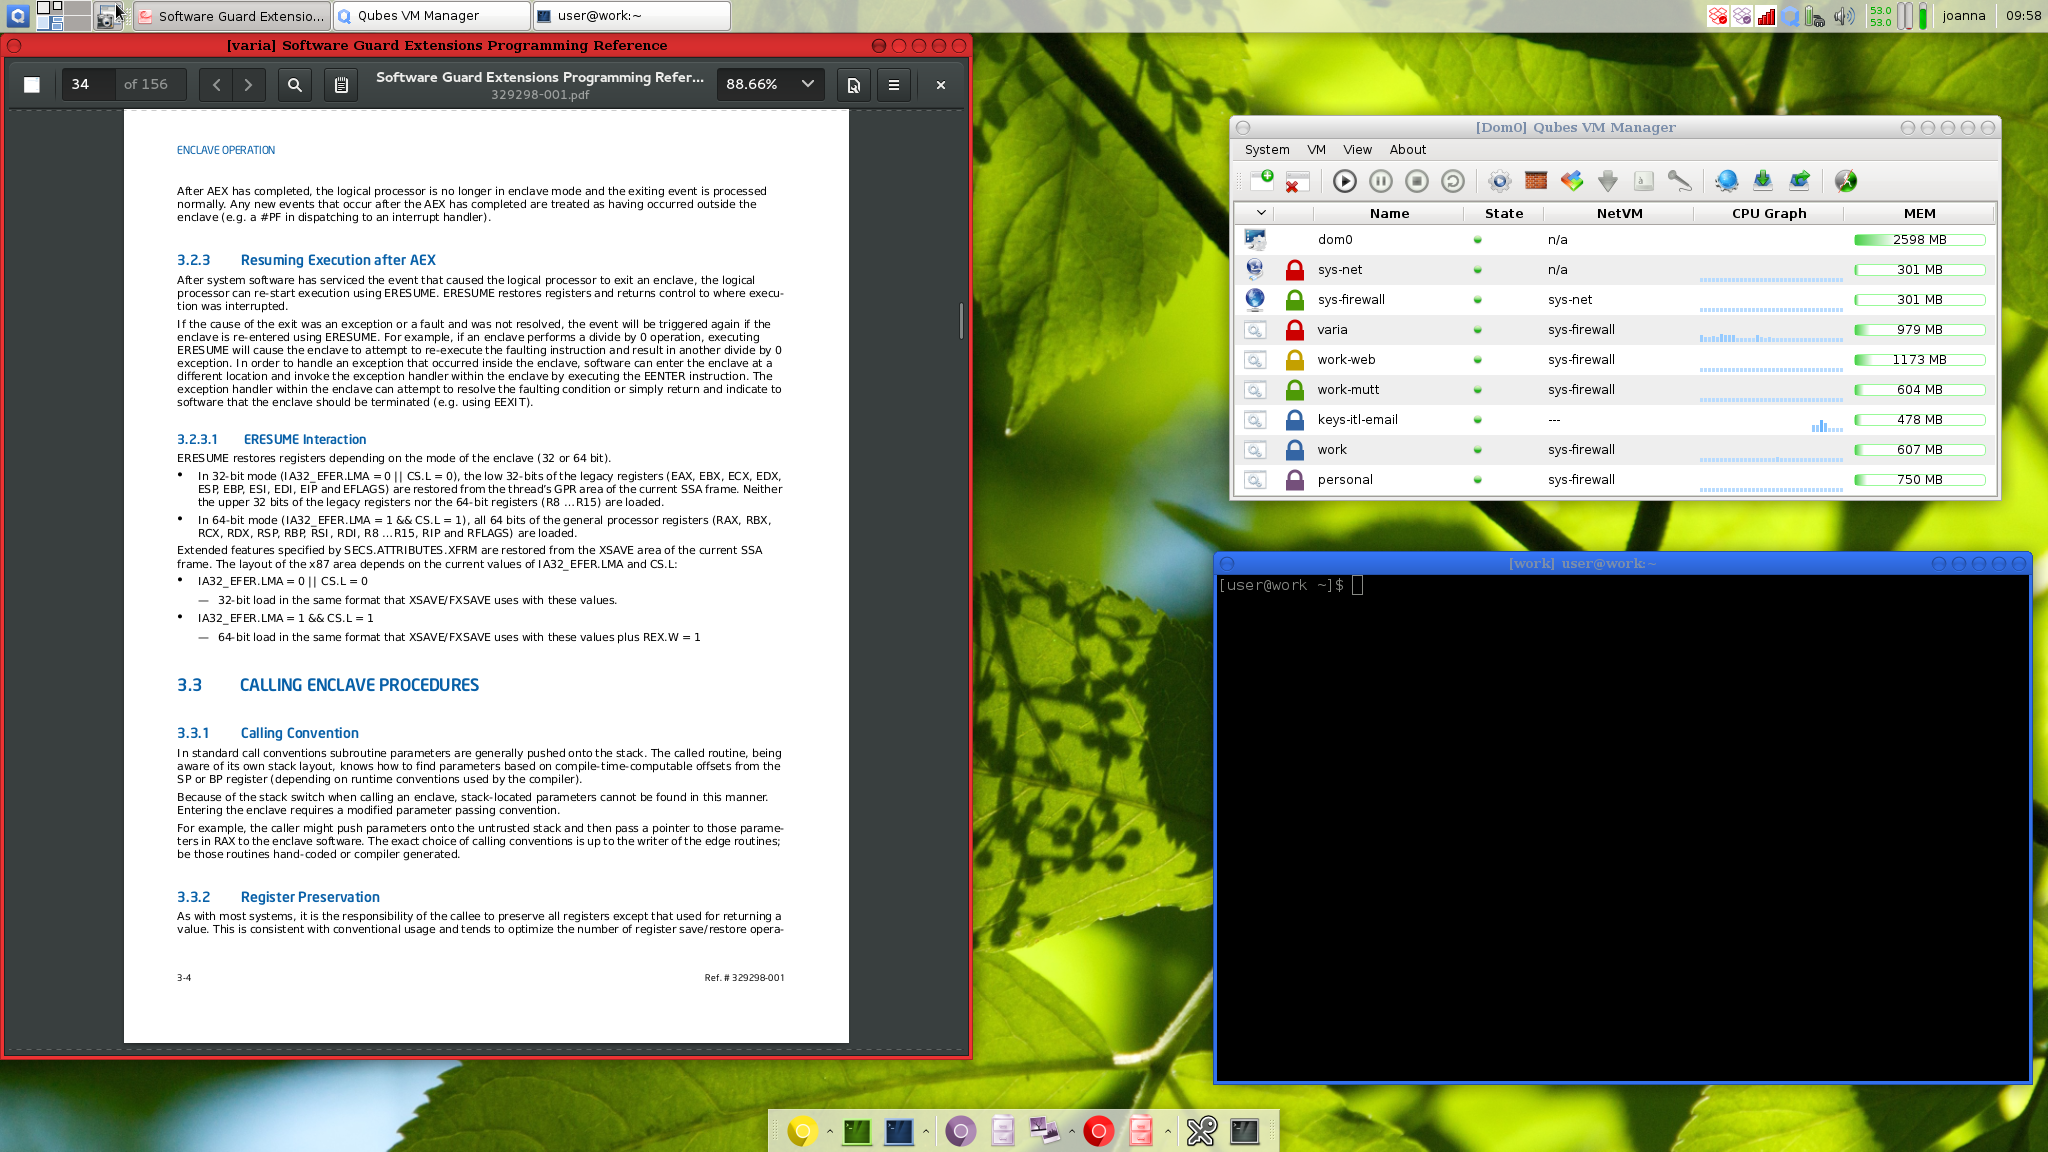
\includegraphics[width=\textwidth]{../sandbox/qubes-desktop1}
\end{frame}




\section{Which sandboxing?}
\begin{frame}{which sandboxing?}
    \begin{itemize}
    \item which whole-application sandboxing technique seems better for 
        \begin{itemize}
        \item security, performance, usability, handling unchanged applications
        \end{itemize}
    \item (full answer: could mix techniques + probably depends on details of app)
    \vspace{.5cm}
    \item A. chroot + system call filtering
    \item B. chroot + mount and user namespaces
    \item C. virtual machine dedicated to application
    \item D. SELinux-like mandatory access control
    \end{itemize}
\end{frame}


\section{sandboxing without OS support}
\begin{frame}{sandboxing without OS support}
    \begin{itemize}
    \item so far: relying on OS features for sandboxing
    \item good reasons:
        \begin{itemize}
        \item primarily want to filter system calls
        \item hardware-assisted, strong protection
        \end{itemize}
    \vspace{.5cm}
    \item but problems with relying on OS:
        \begin{itemize}
        \item sending information in/out of sandbox relatively slow
        \item requires heavily OS-specific code
        \end{itemize}
    \end{itemize}
\end{frame}

\begin{frame}{sandboxing without OS ideas}
    \begin{itemize}
    \item `dynamic' language virtual machine, like Java VM, .Net CLR
        \begin{itemize}
        \item hard to use with code intended to compile to native machine code
        \end{itemize}
    \vspace{.5cm}
    \item virtual machine targetted for C/C++-like code, like WebAssembly
    \vspace{.5cm}
    \item assembly-to-assembly conversion
        \begin{itemize}
        \item example: Wahbe, Lucco, Anderson, and Graham, ``Efficient Software-Based Fault Isolation'' (1993)
        \item example: Ford and Cox, ``Vx32: Lightweight User-level Sandboxing on the x86'' (2008)
        \end{itemize}
    \end{itemize}
\end{frame}


\subsection{Wasm}
\begin{frame}{WebAssembly}
    \begin{itemize}
    \item WebAssembly: language virtual machine specification intended\ldots
        \begin{itemize}
        \item similar idea to Java VM
        \end{itemize}
    \vspace{.5cm}
    \item to be compiled to from C/C++
        \begin{itemize}
        \item support by Clang/LLVM
        \end{itemize}
    \item to be easy to just-in-time compile to native machine code
    \item to be run in web browsers (fast web apps)
    \end{itemize}
\end{frame}

\begin{frame}{WebAssembly memory management}
    \begin{itemize}
    \item WebAssembly `modules' have a single ``linear memory''
    \item starts at index 0, goes to some maximum
    \item load/store instructions take index into current memory
    \vspace{.5cm}
    \item observation 1: close to memory model ``normal'' C/C++ code expects
    \vspace{.5cm}
    \item observation 2: only goal is to prevent sandbox (WebAssembly) code from interfering with outside code
    \item \ldots so no need to check array bound or similar
    \vspace{.5cm}
    \item observation 3: no need to worry about garbage collection
    \end{itemize}
\end{frame}

\begin{frame}{WebAssembly validation}
    \begin{itemize}
    \item WebAssembly virtual machine code designed to be \textit{validated} before running
    \vspace{.5cm}
    \item allows for efficient interpreters or conversion to assembly
        \begin{itemize}
        \item validation ensures that you can safely skip certain type checks, etc.
        \end{itemize}
    \item language specification very explicit about what needs to be checked at runtime
    \end{itemize}
\end{frame}

\begin{frame}{example WebAssembly validation}
    \begin{itemize}
    \item check that instructions have right number of operands available
        \begin{itemize}
        \item WebAssembly instructions use stack (compile \texttt{2 + 2} into \texttt{2 2 +})
        \end{itemize}
    \item check operands that can be checked (constants)
    \item check the calls go to only functions listed in table
        \begin{itemize}
        \item should make it easier to do just-in-time compilation to machine code?
        \end{itemize}
    \item check the branches go to only locations listed in table, and only within one function
        \begin{itemize}
        \item should make it easier to do just-in-time compilation to machine code?
        \end{itemize}
    \end{itemize}
\end{frame}

\begin{frame}{example WebAssembly instruction specification}
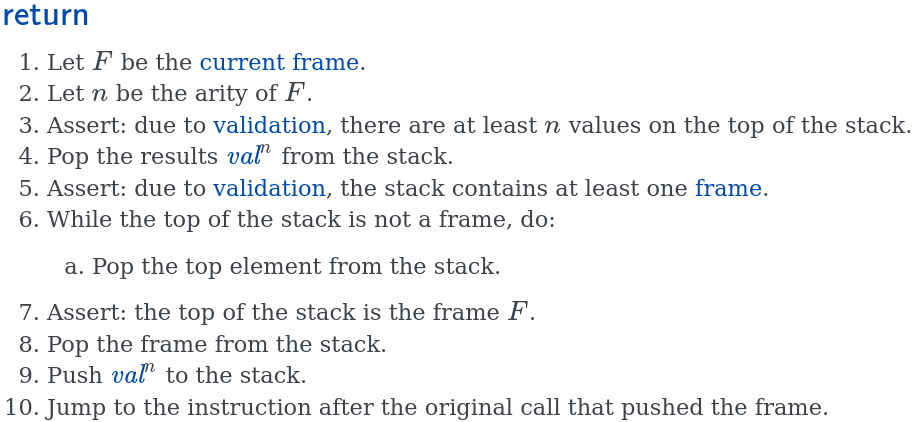
\includegraphics[height=0.8\textheight]{../sandbox/wasm-return-spec}
\end{frame}

\begin{frame}{WebAssembly as sandboxing}
    \begin{itemize}
    \item can compile existing C/C++ library using WebAssembly\ldots
    \item then call using language virtual machine
    \end{itemize}
\end{frame}



\section{sandboxing API: RLBox}
\begin{frame}{RLBox}
    \begin{itemize}
    \item saw interfaces for using sandboxes from user perspective?
    \item what about for privilege separation?
        \begin{itemize}
        \item recall: like Chrome separate renderer process idea
        \item need to navigate OS sandboxing API + create interface for sandboxed part?
        \end{itemize}
    \vspace{.5cm}
    \item some reusable tools have appeared for this (but no clear winner)
    \item one example: RLBox (published in Usenix Security 2020)
        \begin{itemize}
        \item Shravan Narayan and Craig Disselkoen, UC San Diego; Tal Garfinkel, Stanford University; Nathan Froyd and Eric Rahm, Mozilla; Sorin Lerner, UC San Diego; Hovav Shacham, UT Austin; Deian Stefan, UC San Diego
        \end{itemize}
    \end{itemize}
\end{frame}

\begin{frame}[fragile,label=rlboxusage]{RLBox usage}
\begin{itemize}
\item part of example from author's presentation:
    \begin{itemize}
    \item goal: invoke JPEG parser in sandbox
    \end{itemize}
\end{itemize}
\begin{lstlisting}[language=C++,style=script]
autosandbox = rlbox::create_sandbox<wasm>();
tainted<jpeg_decompress_struct*> p_jpeg_img = sandbox.malloc_in_sandbox<jpeg_decompress_struct>();
tainted<jpeg_source_mgr*> p_jpeg_input_source_mgr = sandbox.malloc_in_sandbox<jpeg_source_mgr>();
sandbox.invoke(jpeg_create_decompress, p_jpeg_img);
p_jpeg_img->src = p_jpeg_input_source_mgr;
p_jpeg_img->src->fill_input_buffer = ...;
sandbox.invoke(jpeg_read_header,p_jpeg_img/*...*/);
\end{lstlisting}
\begin{itemize}
\item tool handles running `jpeg\_create\_decompress', `jpeg\_read\_header' in sandbox
\item values shared with sandbox marked as ``tainted''
    \begin{itemize}
    \item C++ (template) class
    \end{itemize}
\item this example: using WebAssembly-based sandbox
\item used in firefox
\end{itemize}
\end{frame}


\section{application permissions}
\usetikzlibrary{calc}
\begin{frame}{some Android prompts}
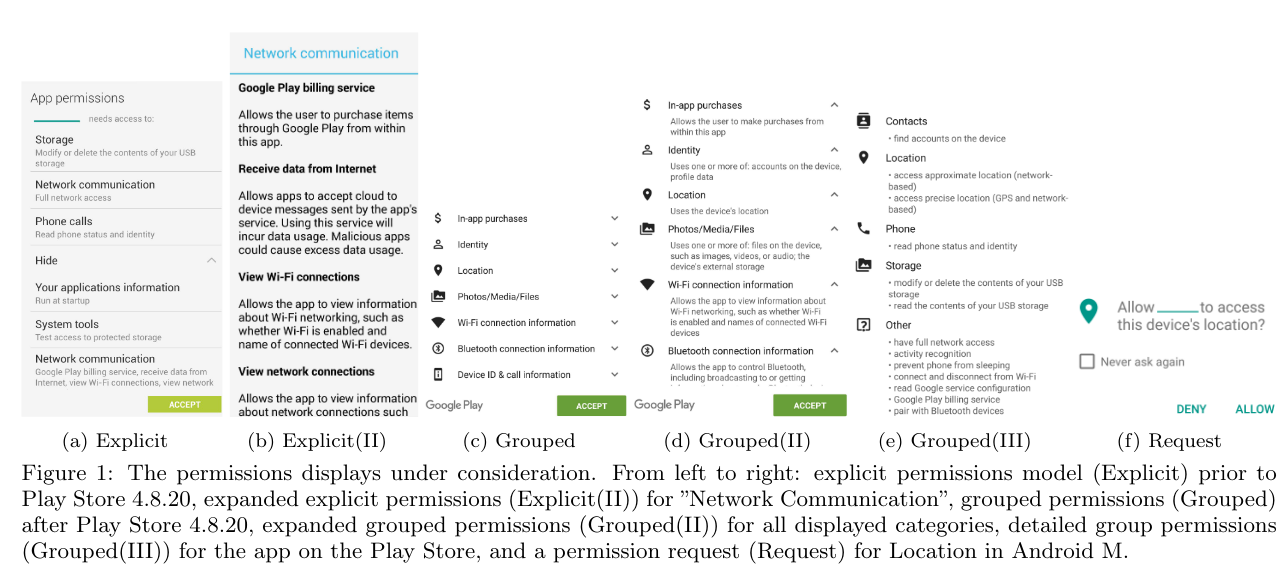
\includegraphics[width=\textwidth]{../sandbox/android-perm-screens}
\imagecredit{from Clark et al, ``No Time At All: Opportunity Cost of Android Permissions'' (HotWireless'16)}
\end{frame}


\subsection{UI problems}

\begin{frame}<1>[label=appPermUI]{UI problems with application permissions}
    \begin{itemize}
    \item \myemph<2>{do applications request sensible permissions?}
    \item \myemph<3>{do users pay attention to permission requests?}
    \item \myemph<3>{do users understand what permissions mean?}
    \item are permissions fine-grained enough?
    \item are permissions coarse-grained enough?
    \end{itemize}
\end{frame}


\subsection{do request right permissions?}
\againframe<2>{appPermUI}
\begin{frame}{right permissions?}
    \begin{itemize}
    \item Felt, Chin, Hanna, Song and Wagner, ``Android Permissions Demystified'' (CCS 2011)
    \item used static analysis to compare requested permissions to what applications did
        \begin{itemize}
        \item at the time: permissions requested at installation
        \end{itemize}
    \item sample of 900 applications
    \item estimate approx 200 over-privileged
        \begin{itemize}
        \item (estimate because using false positive rate from manual checking)
        \end{itemize}
    \end{itemize}
\end{frame}

\begin{frame}{why extra permissions?}
    \begin{itemize}
    \item selected from Felt et al's analysis:
    \item developers confused similar permissions
        \begin{itemize}
        \item \texttt{ACCESS\_NETWORK\_STATE} versus \texttt{ACCESS\_WIFI\_STATE}
        \end{itemize}
    \item developers thought permissions were needed for delegated tasks
        \begin{itemize}
        \item \texttt{CALL\_PHONE} not needed to invoke phone app
        \item \texttt{INSTALL\_APPLICATION} not needed to open app store install dialog
        \end{itemize}
    \item developers thought permissions needed for all methods of class
        \begin{itemize}
        \item \texttt{WRITE\_SETTINGS} when using (no-permission) read-settings operations
        \end{itemize}
    \item copy-and-paste
    \end{itemize}
\end{frame}


\subsection{do users understand permissions?}
\againframe<3>{appPermUI}
\begin{frame}{a user study (2012)}
    \begin{itemize}
    \item Felt, Ha, Egelman, Haney, Chin, Wagner, ``Android Permissions: User Attention, Comprehension, and Behavior''
    \item performed lab study; task: find + install coupon app
    \item at the time: Android prompted for permissions on installation
    \vspace{.5cm}
    \item<2-> 17\% looked at app permissions detail
    \item<2-> 42\% aware of permissions
    \item<2-> 42\% unaware of permissions
    \vspace{.5cm}
    \item<2-> versus: 88\% read reviews 
    \end{itemize}
\end{frame}

\begin{frame}{a user survey (2012)}
    \begin{itemize}
    \item same paper did survey about what permissions meant
    \item three multiple choice questions 
        \begin{itemize}
        \item selected from bank of 11
        \end{itemize}
    \item 302 respondents; 3 fully correct
    \item average 21\%
    \end{itemize}
\end{frame}

\begin{frame}{example survey question}
    \begin{itemize}
    \item `Read phone state and identity' allows which of these?
    \vspace{.5cm}
    \item Read your phone number
    \item See who you have called
    \item Track you across applications
    \item Load adverisements
    \end{itemize}
\end{frame}

\begin{frame}{survey questions (1)}
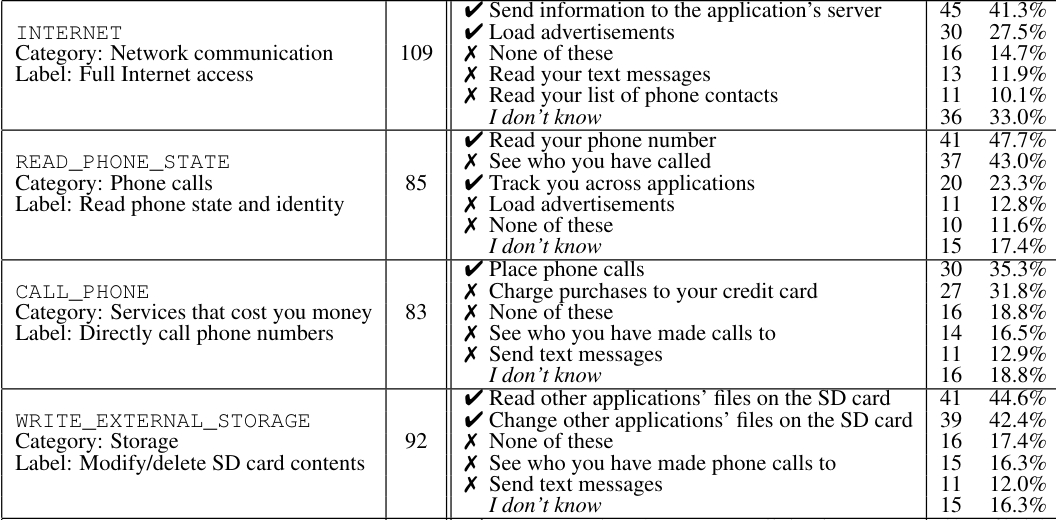
\includegraphics[width=\textwidth]{../sandbox/android-perm-survey1}
\end{frame}

\begin{frame}{survey questions (2)}
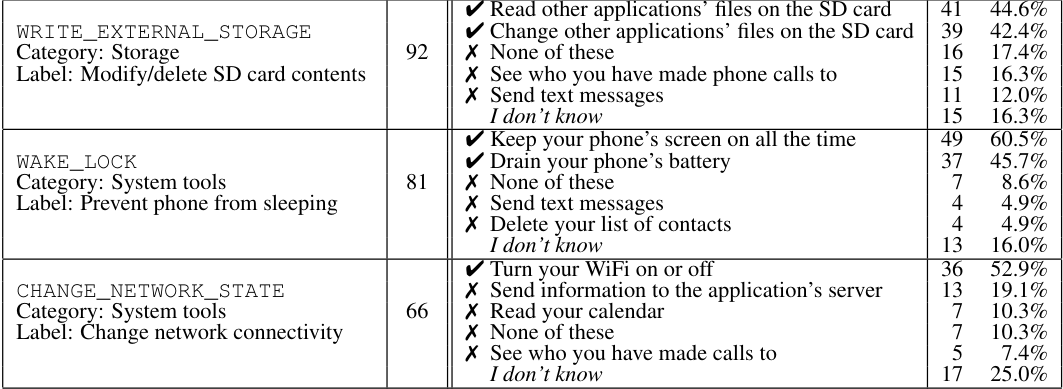
\includegraphics[width=\textwidth]{../sandbox/android-perm-survey2}
\end{frame}

\begin{frame}{survey questions (3)}
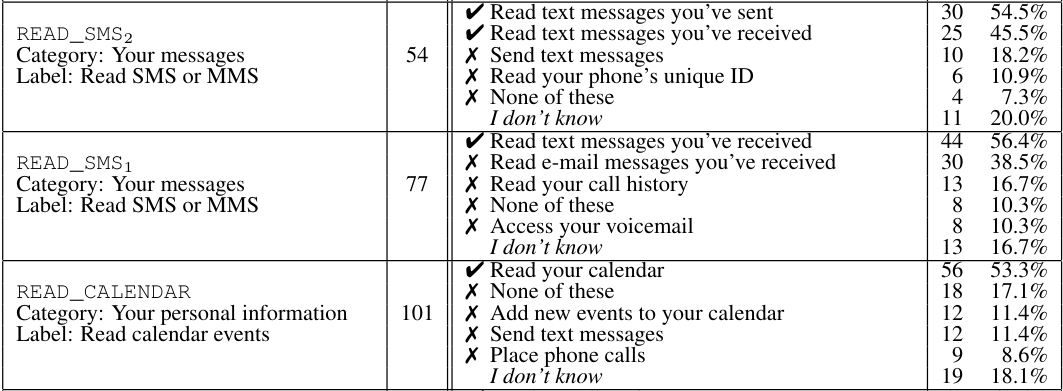
\includegraphics[width=\textwidth]{../sandbox/android-perm-survey3}
\end{frame}

\begin{frame}{survey questions (4)}
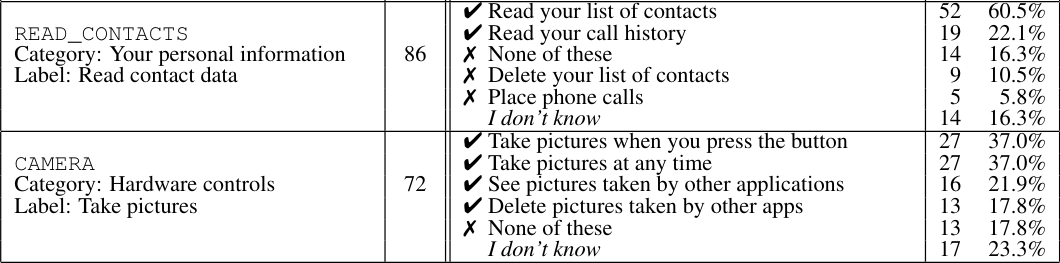
\includegraphics[width=\textwidth]{../sandbox/android-perm-survey4}
\end{frame}


\subsection{how to ask for permission?}
\begin{frame}
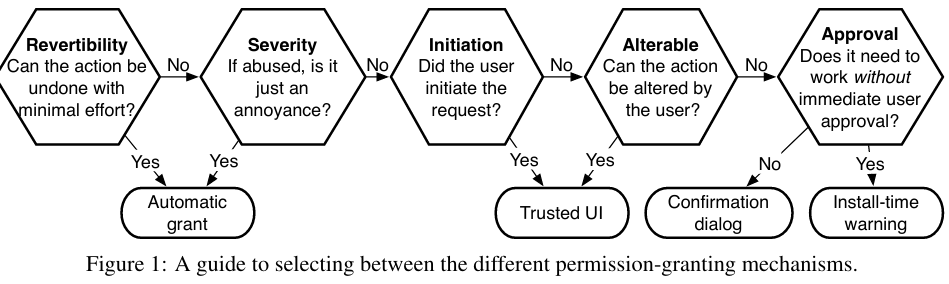
\includegraphics[width=\textwidth]{../sandbox/app-perm-how}
\scriptsize from Felt et al, ``How To Ask For Permission'' (HotSec'12)
\end{frame}

\begin{frame}{principles}
    \begin{itemize}
    \item Felt et al list ``principles'':
    \vspace{.5cm}
    \item ``Conserve user attention, utilizaing it for only permissions that have severe consquences''
        \begin{itemize}
        \item too many security warnings means users won't pay attention
        \end{itemize}
    \item ``When possible, avoid interrupting the user's primary task with explicit security decisions''
        \begin{itemize}
        \item users will dismiss warnings because they get in the way of work
        \end{itemize}
    \end{itemize}
\end{frame}


\subsection{permissions abuse: Cloak and Dagger}
\begin{frame}{Cloak and Dagger}

\includegraphics[width=\textwidth]{../sandbox/cloak-and-dagger}
\end{frame}

\begin{frame}{cloak and dagger permissions}
    \begin{itemize}
    \item the two permissions:
        \begin{itemize}
        \item SYSTEM\_ALERT\_WINDOW: \\
            draw windows on top of screen \\
            (at time: enabled by default)
        \item BIND\_ACCESSIBILITY\_SERVICE: \\
            ``Observe your actions'' \\
            ``Retrieve window content''
        \end{itemize}
    \item can hide window content while user interacts with it
    \item \ldots and stealthy get user to do more things
    \end{itemize}
\end{frame}

\begin{frame}{also, a clickjacking attack}
    \begin{itemize}
    \item at the time, could draw overlay window over permissions dialog
    \item \ldots convince user to press where ``OK'' button is
    \item countermeasure: permissions dialog would detect this, ignore clicks
    \vspace{.5cm}
    \item problem: wouldn't detect if overlay didn't cover enough of button
    \end{itemize}
\end{frame}


\subsection{permissions abuse: information leak}
\begin{frame}{privacy and permissions}
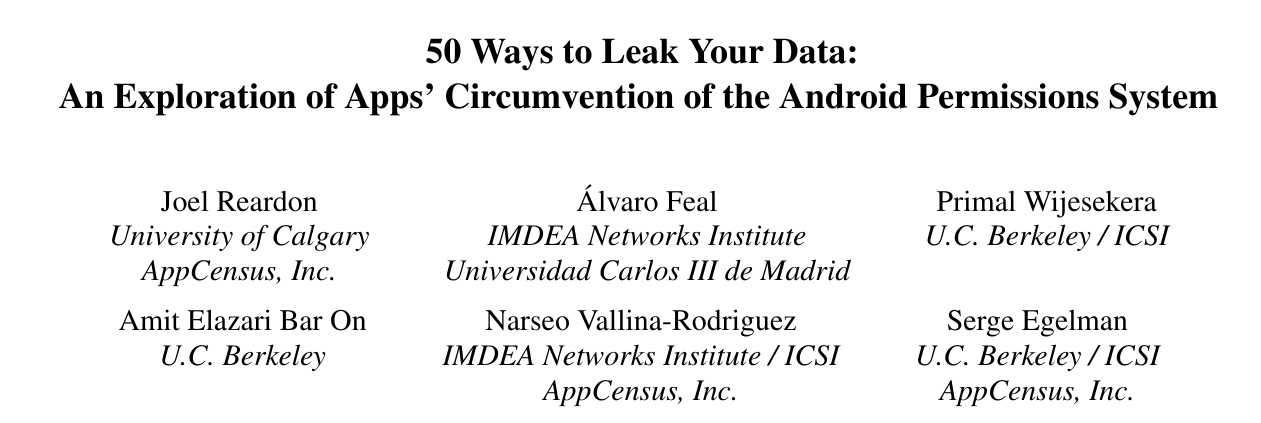
\includegraphics[width=0.7\textwidth]{../sandbox/priv-and-perm}
    \begin{itemize}
    \item 2019 paper
    \item many mobile application permissions related to privacy
    \item getting phone ID, email address, location, \ldots
    \item but applications (especially ad libraries) find workarounds
    \end{itemize}
\end{frame}

\begin{frame}{permissions being insufficient}
    \begin{itemize}
    \item permissions check limited API calls for getting private info,\ldots
    \item \ldots but there were alternative, unfiltered system calls for
    \vspace{.5cm}
    \item getting MAC address (effectively phone ID)
        \begin{itemize}
        \item Linux \texttt{ioctl} system call on socket
        \end{itemize}
    \item WiFi base station address
        \begin{itemize}
        \item ARP cache (recently seen machines on network, to know where to send packets)
        \end{itemize}
    \item location
        \begin{itemize}
        \item geolocation tag on recent photos
        \end{itemize}
    \end{itemize}
\end{frame}

\begin{frame}{covert channels}
    \begin{itemize}
    \item advertising libraries would store phone ID/account info in a file
        \begin{itemize}
        \item \ldots when they had permissions to retrieve it
        \end{itemize}
    \item and would read phone ID/account info from a file
        \begin{itemize}
        \item \ldots when they did not
        \end{itemize}
    \end{itemize}
\end{frame}


% FIXME: sandboxing and UIs


% FIXME: https://www.usenix.org/system/files/sec19-reardon.pdf
% FIXME: SFI and/or WAsm

\usetikzlibrary{calc}

\section{adding bounds checking}
\begin{frame}{so far}
    \begin{itemize}
    \item many vulnerabilities we looked at due to poor bounds checking
        \begin{itemize}
        \item one exception: use-after-free and related
        \end{itemize}
    \vspace{.5cm}
    \item can we just fix this?
    \end{itemize}
\end{frame}


\subsection{compiler-added?}

\begin{frame}[fragile,label=fortifyMemCpyIntro]{adding bounds checking}
\lstset{language=C,style=small}
\begin{lstlisting}
char buffer[42];
memcpy(buffer, attacker_controlled, len);
\end{lstlisting}
    \begin{itemize}
        \item couldn't compiler add check for \texttt{len}
        \item modern Linux: it does
    \end{itemize}
\end{frame}

\begin{frame}[fragile,label=boundsChecking]{added bounds checking}
\lstset{language=C,style=small}
\begin{lstlisting}
char buffer[42];
memcpy(buffer, attacker_controlled, len);
\end{lstlisting}
\lstset{language=myasm,style=small}
\begin{lstlisting}
    subq   $72, %rsp
    leaq   4(%rsp), %rdi
    movslq len, %rdx
    movq   attacker_controlled, %rsi
    movl   $42, %ecx
    call   __memcpy_chk
\end{lstlisting}
    \begin{itemize}
        \item length \texttt{42} passed to \texttt{\_\_memcpy\_chk}
    \end{itemize}
\end{frame}

\begin{frame}{\_FORTIFY\_SOURCE}
    \begin{itemize}
        \item Linux C standard library + GCC features
        \item adds automatic checking to a bunch of string/array functions
        \item also printf (disable \texttt{\%n} unless format string is a constant)
        \vspace{.5cm}
        \item often enabled by default
        \item GCC options:
            \begin{itemize}
                \item \texttt{-D\_FORTIFY\_SOURCE=1} --- enable (backwards-compatible only)
                \item \texttt{-D\_FORTIFY\_SOURCE=2} --- enable (constant sizes only)
                \item \texttt{-D\_FORTIFY\_SOURCE=3} --- enable (computed sizes, sometimes)
                \item \texttt{-U\_FORTIFY\_SOURCE} --- disable
            \end{itemize}
    \end{itemize}
\end{frame}


\begin{frame}[fragile,label=fortifySrcExample]{bounds checking will happen...}
will add checks (gcc 9.3 \textbf{-O2}, FORTIFY\_SOURCE=1/2)
\begin{lstlisting}[language=C,style=smaller]
void example1() {
    char dest1[1024]; memcpy(dest1, ...); ...
}
char dest2[1024];
void example2() {
    memcpy(dest2, ...); ...
}
void example3() {
    char *p = &dest2[4]; memcpy(p, ...); ...
}
\end{lstlisting}
\end{frame}

\begin{frame}[fragile,label=fortifySrcExample2]{bounds checking will happen...}
will add checks (gcc 14.2 or clang 20 \textbf{-Os}, FORTIFY\_SOURCE=3)
\begin{lstlisting}[language=C,style=smaller]
char dest2[1024];
void example4() {
    char *p = &dest2[mystery()]; memcpy(p, ...); ...
}
\end{lstlisting}
\begin{itemize}
\item no checking with FORTIFY\_SOURCE=2
\item extra overhead: computing min(50, 1024-mystery())
\end{itemize}
\end{frame}

\begin{frame}[fragile,label=fortifySrcExample3]{bounds checking will happen...}
will add check (gcc 14.2 or clang 20 \textbf{-Os}, FORTIFY\_SOURCE=3)
\begin{lstlisting}[language=C,style=smaller]
char dest2[1024];
void example5() {
    char dest3[128];
    char *p = dest2;
    if (mystery()) p = dest3;
    memcpy(p, ...); ...
}
\end{lstlisting}
\begin{itemize}
\item checks for maximum possible with FORTIFY\_SOURCE=2
\end{itemize}
\end{frame}

\begin{frame}[fragile,label=fortifySourceExample4]{bounds checking won't happen...}
\begin{lstlisting}[language=C,style=smaller]
char dest2[1024];
struct Foo {
    char buffer1[128];
    int *pointer;
    ...
};
void example6(struct Foo *f, int size) {
    memcpy(f->buffer1, dest2, size);
}
\end{lstlisting}
\end{frame}

\begin{frame}[fragile,label=fortifySourceExample4]{bounds checking won't quite happen...}
\begin{lstlisting}[language=C,style=smaller]
char dest2[1024];
struct Foo {
    char buffer1[128];
    int *pointer;
    ...
};
struct Foo f;
void example6(int size) {
    memcpy(f.buffer1, dest2, size);
}
\end{lstlisting}
\begin{itemize}
\item checks that size is less than sizeof(struct Foo) (not 128)
\end{itemize}
\end{frame}

\begin{frame}{implementation}
    \begin{itemize}
    \item GCC/clang expose `object size` and `dynamic object size' function
    \item relies on compiler analysis to know size from see declaration or malloc/etc. assignemnt
    \vspace{.5cm}
    \item limited
    \end{itemize}
\end{frame}

\subsection{and library functions}
        % FIXME: exercise: what should call have been
            % needs answers

\begin{frame}[fragile,label=nonChecking]{non-checking library functions}
\lstset{language=C,style=small}
    \begin{itemize}
    \item some C library functions make bounds checking hard: 
\begin{lstlisting}
strcpy(dest, source);
strcat(dest, source);
sprintf(dest, format, ...);
\end{lstlisting}
    \item bounds-checking versions (\myemph{added to library later}):
\begin{lstlisting}
/* might not add \0 (!) */
strncpy(dest, source, size);
strncat(dest, source, size);
snprintf(dest, size, format, ...);
\end{lstlisting}
    \end{itemize}
\end{frame}

\begin{frame}[fragile,label=poorBoundsChecking]{poor bounds-checking APIs}
\begin{lstlisting}[language=C,style=smaller]
char dest[100];
/* THIS CODE IS BROKEN */
strncpy(dest, source1, sizeof dest);
strncat(dest, source2, sizeof dest);
printf("result was %s\n", dest)
\end{lstlisting}
\begin{itemize}
\item the above can access memory of out of bounds
\item \ldots in a bunch of ways
\end{itemize}
\end{frame}

\begin{frame}[fragile,label=strncpyManual]{Linux's strncpy manual}
\begin{lstlisting}[language=C,style=smaller]
strncpy(dest, source1, sizeof dest);
\end{lstlisting}
\begin{itemize}
\item ``Warning: If there is no
       null byte among the first n bytes of src, the string placed in dest will not be null-terminated.''
\end{itemize}
\begin{itemize}
\item exercise: what should the call have been?
\end{itemize}
\end{frame}


\begin{frame}[fragile,label=strncatManual]{Linux's strncat manual}
\begin{lstlisting}[language=C,style=smaller]
strncat(dest, source2, sizeof dest);
\end{lstlisting}
\begin{itemize}
\item ``If src contains n or more bytes, strncat() writes n+1 bytes to  dest  (n
from  src  plus the terminating null byte).  Therefore, the size of dest
must be at least strlen(dest)+n+1.''
\end{itemize}
\begin{itemize}
\item exercise: what should the call have been?
\end{itemize}
\end{frame}

\begin{frame}[fragile,label=betterStrX]{better versions?}
\begin{itemize}
\item FreeBSD (and Linux via libbsd): strlcpy, strlcat
\item ``Unlike [strncat and strncpy], strlcpy() and strlcat() take the full size of the buffer
        and gaurenteeto NUL-terminate the result...''
\end{itemize}
\begin{lstlisting}[language=C++,style=smaller]
strlcpy(dest, source1, sizeof dest);
strlcat(dest, source2, sizeof dest);
\end{lstlisting}
\vspace{.5cm}
\begin{itemize}
\item Windows: \texttt{strcpy\_s}, \texttt{strcat\_s} (same idea, differentname)
\end{itemize}
\end{frame}

\begin{frame}[fragile,label=cppBounds]{C++/Rust bounds checking}
\lstset{language=C,style=small}
\begin{lstlisting}
#include <vector>
...
std::vector<int> data;
data.resize(50);
// undefined behavior:
data[60] = 0;
// throws std::out_of_range exception
data.at(60) = 0;
\end{lstlisting}
\vspace{-\baselineskip}
\hrulefill
\begin{Verbatim}[fontsize=\small]
let data: Vec<i32> = ...;
data.resize(50, 0);
// undefined behavior:
unsafe { *data.get_unchecked_mut(60) = 1; }
// panics at runtime:
data[60] = 0;  
\end{Verbatim}
\end{frame}



\subsection{language support?}


\begin{frame}{language-level solutions}
    \begin{itemize}
    \item languages like Python don't have this problem
    \item couldn't we do the same thing in C?
    \end{itemize}
\end{frame}




\subsection{simple case for bounds checking in C}
\begin{frame}{bounds-checking C}
    \begin{itemize}
    \item there have been many proposals to add bounds-checking to C
    \item including implementations
    \item brainstorm: \myemph{why hasn't this happened?}
    \end{itemize}
\end{frame}

\begin{frame}[fragile,label=addBounds]{easy bounds-checking}
    \lstset{language=C,style=smaller}
\begin{lstlisting}
void vulnerable() {
    char buffer[100];
    int c;
    int i = 0;
    while ((c = getchar()) != EOF && c != '\n') {
        buffer[i] = c;
    }
}
void vulnerable_checked() {
    char buffer[100];
    int c;
    int i = 0;
    while ((c = getchar()) != EOF && c != '\n') {
        FAIL_IF(i >= 100 || i < 0);
        buffer[i] = c;
    }
}
\end{lstlisting}
\end{frame}


\subsection{the problematic case}
\begin{frame}[fragile,label=addBoundsHarder]{harder bounds-checking}
    \lstset{language=C,style=smaller}
\begin{lstlisting}
void vulnerable(char *buffer) {
    char buffer[100];
    int c;
    int i = 0;
    while ((c = getchar()) != EOF && c != '\n') {
        buffer[i] = c;
    }
}
void vulnerable_checked(char *buffer) {
    int c;
    int i = 0;
    while ((c = getchar()) != EOF && c != '\n') {
        FAIL_IF(i >= UNKNOWN || i < UNKNOWN);
        buffer[i] = c;
    }
}
\end{lstlisting}
\end{frame}


\subsection{fat pointer idea}
% FIXME: smoother transition
    % FIXME: exercise about problematic cases


\begin{frame}[fragile,label=wrappedPointers]{adding bounds-checking --- fat pointers}
\lstset{
    language=C,
    style=small
}
\begin{lstlisting}
struct MyPtr {
    char *pointer; /* "raw" pointer value */
    char *minimum; /* first byte of buffer pointed to */
    char *maximum; /* last byte of buffer pointed to */
};
\end{lstlisting}
\begin{visibleenv}<2->
\hrule
\begin{lstlisting}
char buffer[100];
char *p = &buffer[10];
\end{lstlisting}
becomes
\begin{lstlisting}
char buffer[100];
MyPtr p = {
    .pointer = &buffer[10],
    .minimum = &buffer[0],
    .maximum = &buffer[99]
};
\end{lstlisting}
\end{visibleenv}
\end{frame}



\subsubsection{strcpy example}
\begin{frame}[fragile,label=wrappedPtrStrcpy]{adding bounds checking --- strcpy}
\lstset{
    language=C,
    style=small
}
\begin{lstlisting}
MyPtr strcpy(MyPtr dest, const MyPtr src) {
    int i;
    do {
        CHECK(src.pointer + i <= src.maximum);
        CHECK(src.pointer + i >= src.minimum);
        CHECK(dest.pointer + i <= dest.maximum);
        CHECK(dest.pointer + i >= dest.minimum);
        dest.pointer[i] = src.pointer[i];
        i += 1;
        CHECK(src.pointer + i <= src.maximum);
        CHECK(src.pointer + i >= src.minimum);
    } while (src.pointer[i] != '\0');
    return dest;
}
\end{lstlisting}
\end{frame}




\subsubsection{overhead?}

\begin{frame}{speed of bounds checking}
    \begin{itemize}
    \item two comparisons for every pointer access?
    \item three times as much space for every pointer?
    \end{itemize}
\end{frame}



\subsection{unfortunate things C programmers do}
\begin{frame}[fragile,label=unfortunateCProg1]{unfortunate things C programmers do (1)}
from FreeBSD's bootpd (server for machines that boot from the network):
\begin{lstlisting}[language=C,style=smaller]
struct shared_string {
    unsigned int linkcount;
    char         string[1]; /* Dynamically extended */
};
...
s = (struct shared_string *) smalloc(
        sizeof(struct shared_string) + length
    );
...
\end{lstlisting}
\end{frame}

\begin{frame}[fragile,label=unfortunateCProg2]{unfortunate things C programmers do (2)}
from perl's source code:
\begin{lstlisting}[language=C,style=small]
sv_setuv(my_pool_sv, PTR2UV(my_poolp));
...
/* later, in another function: */
my_pool_t *my_poolp = INT2PTR(my_pool_t*, SvUV(my_pool_sv));
\end{lstlisting}
\begin{itemize}
\item PTR2UV: pointer to Unsigned int Value
\item INT2PTR: integer to pointer value
\end{itemize}
\end{frame}

\begin{frame}[fragile,label=unfortunateCProg3]{unfortunate things C programmers do (3)}
\begin{lstlisting}[language=C,style=small]
struct SuperClass;
struct SubClass {
    struct SuperClass super;
    ...
}

struct SubClass sub;
struct SuperClass *super = &sub.super;
some_function(super);
...
some_function(struct SuperClass *super) {
    ...
    struct SubClass *sub = (struct SubClass *)super;
    ...
}
\end{lstlisting}
\end{frame}



\subsection{fat pointers in reality?}
\begin{frame}{example: CCured}
\begin{itemize}
\item Necula et al, ``CCured:  Type-Safe Retrofitting of Legacy Code'' (2002)
\vspace{.5cm}
\item extension to C to add fat pointers
\item actually three different types of pointers:   
    \begin{itemize}
    \item SAFE: point to single object (not array) or NULL
    \item SEQUENCE: pointer to array with known bounds (like ``fat'' pointers)
    \item DYNAMIC: extra to handles type-casting
    \end{itemize}
\item \textit{needs source changes} to annotate some pointer usage
    \begin{itemize}
    \item especially to allow library function calls
    \end{itemize}
\item 1-\textbf{2.5x} time overhead
\end{itemize}
\end{frame}


\section{baggy bounds checking}

\begin{frame}{research example (2009)}
    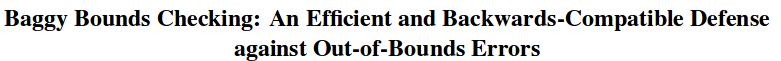
\includegraphics[width=\textwidth]{../bounds/baggy-bounds-title}
\end{frame}

\begin{frame}[fragile,label=lookupTable]{baggy bounds checking idea}
    \begin{itemize}
        \item giant lookup table --- one entry for every 16 bytes of memory
        \item table indicates start of object allocated here
        \item check pointer arithmetic:
    \end{itemize}
\begin{lstlisting}
char p = str[i];
/* becomes: */
CHECK(START_OF[str / 16] == START_OF[&str[i] / 16]);
char p = str[i];
\end{lstlisting}
\end{frame}




\subsection{trick for good performance}

\begin{frame}[fragile,label=baggyBoundsTrick]{baggy bounds trick}
\lstset{language=C,style=small}
    \begin{itemize}
        \item table of pointers to starting locations would be huge
        \item add some restrictions:
            \begin{itemize}
            \item all object sizes are powers of two
            \item all object starting addresses are a multiple of their size
            \end{itemize}
        \item then, table contains size info only:
            \begin{itemize}
            \item table contains $i$, size is $2^i$ bytes:
            \end{itemize}
    \end{itemize}
\begin{lstlisting}
char *GetStartOfObject(char *pointer) {
    return pointer & ~(1 << TABLE[pointer / 16] - 1);
    /* pointer bitwise-and 2^(table entry) - 1 */
    /* clear lower (table entry) bits  of pointer */
}
\end{lstlisting}
\end{frame}



\subsection{the lookup table}
\usetikzlibrary{fit,matrix}

\tikzset{
    stackBox/.style={very thick},
    allocBox/.style={dashed,very thick,fill=blue!20},
    onStack/.style={thick},
    frameOne/.style={fill=blue!15},
    frameTwo/.style={fill=red!15},
    markLine/.style={blue!50!black},
    markLineB/.style={red!90!black},
    hiLine/.style={red!90!black},
}
\begin{frame}<1-6>[fragile,label=lkpTble]{allocations and lookup table}
    \begin{tikzpicture}
        \draw[onStack] (0, 0) rectangle (4, -7);
        \draw[allocBox] (0, 0) rectangle (4, -0.4);
        \draw[stackBox] (0, 0) rectangle (4, -0.5);
        \draw[allocBox] (0, -0.5) rectangle (4, -0.8);
        \draw[stackBox] (0, -0.5) rectangle (4, -1.0);
        \draw[allocBox] (0, -1) rectangle (4, -1.9);
        \draw[stackBox] (0, -1) rectangle (4, -2);
        \draw[allocBox] (0, -2) rectangle (4, -2.4);
        \draw[stackBox] (0, -2) rectangle (4, -2.5);
        \draw[allocBox] (0, -2.5) rectangle (4, -2.7);
        \draw[stackBox] (0, -2.5) rectangle (4, -3);
        \draw[stackBox] (0, -3) rectangle (4, -4);
        \draw[allocBox] (0, -4) rectangle (4, -5.2);
        \draw[stackBox] (0, -4) rectangle (4, -6);

        \begin{visibleenv}<1->
            \node[anchor=north west,align=left] at (9, 0) {
                object allocated in \\ \myemph<1>{power-of-two `slots'}
            };
        \end{visibleenv}
        \begin{visibleenv}<2->
            \matrix[tight matrix,
                nodes={text width=1cm,font=\small\tt},anchor=north west,label={north:table}] (tbl) at (7, -1) {
                $2^4$ \\ $2^4$  \\ $2^5$ \\ $2^5$ \\ $2^4$ \\ $2^4$ \\
                $0$ \\ $0$ \\
                $2^6$ \\ $2^6$ \\ $2^6$ \\ $2^6$ \\
            };
            \begin{scope}[thick,dotted,-Latex]
            \draw (4, -.25) -- (tbl-1-1.west);
            \draw (4, -.75) -- (tbl-2-1.west);
            \draw (4, -1.25) -- (tbl-3-1.west);
            \draw (4, -1.75) -- (tbl-4-1.west);
            \draw (4, -2.25) -- (tbl-5-1.west);
            \draw (4, -2.75) -- (tbl-6-1.west);
            \draw (4, -3.25) -- (tbl-7-1.west);
            \draw (4, -3.75) -- (tbl-8-1.west);
            \draw (4, -4.25) -- (tbl-9-1.west);
            \end{scope}
        \end{visibleenv}
        \begin{visibleenv}<3>
            \draw[ultra thick,red] (0, -1) rectangle (4, -2);
            \node[draw,ultra thick,red,inner sep=0mm,fit=(tbl-3-1) (tbl-4-1)] {};
            \draw[ultra thick,blue] (0, -4) rectangle (4, -6);
            \node[draw,ultra thick,blue,inner sep=0mm,fit=(tbl-9-1) (tbl-12-1)] {};
        \end{visibleenv}
        \begin{visibleenv}<3->
            \node[anchor=north west,align=left] at (9, -2) {
                table stores sizes \\
                \myemph{for each 16 bytes}
            };
        \end{visibleenv}
        \begin{visibleenv}<4>
            \draw[ultra thick,red] (0, -3) rectangle (4, -4);
            \node[draw,ultra thick,red,inner sep=0mm,fit=(tbl-7-1) (tbl-8-1)] {};
        \end{visibleenv}
        \begin{visibleenv}<4->
            \node[anchor=north west,align=left] at (9, -3.5) {
                addresses \textbf<4>{multiples of size} \\
                (may \myemph{require padding})
            };
        \end{visibleenv}
        \begin{pgfonlayer}{bg}
        \begin{visibleenv}<5>
            \fill[red!30] (0, -5.2) rectangle (4, -6.);
            \fill[red!30] (0, -2.7) rectangle (4, -3.);
            \fill[red!30] (0, -1.9) rectangle (4, -2.);
            \fill[red!30] (0, -2.4) rectangle (4, -2.5);
            \fill[red!30] (0, -0.8) rectangle (4, -1.);
            \fill[red!30] (0, -0.4) rectangle (4, -0.5);
        \end{visibleenv}
        \end{pgfonlayer}
        \begin{visibleenv}<5->
            \node[anchor=north west,align=left] at (9, -5.5) {
                sizes are \textbf<5>{powers of two} \\
                (may \myemph{require padding})
            };
        \end{visibleenv}
    \end{tikzpicture}
\end{frame}

\begin{frame}[fragile,label=managing]{managing the table}
    \begin{itemize}
        \item not just done \texttt{malloc()/new}
        \item also for stack allocations:
    \end{itemize}
    \begin{lstlisting}[style=small,language=C]
void vulnerable() {
    char buffer[100];
    gets(vulnerable);
}
\end{lstlisting}
    \begin{tikzpicture}[remember picture, overlay]
        \node[anchor=north east] at ([xshift=-.25cm, yshift=-1cm]current page.north east) {
    \begin{lstlisting}[style=small,language=myasm]
vulnerable:
  // make %rsp a multiple
  // of 128 (2^7) 
  andq $0xFFFFFFFFFFFFFF80, %rsp
  // allocate 128 bytes
  subq $0x80, %rsp
  // rax <- rsp / 16
  movq $rsp, %rax
  shrq $4, %rax
  movb $7, TABLE(%rax)
  movb $7, TABLE+1(%rax)
  ...
  movq %rsp, %rdi
  call gets
  ret
\end{lstlisting}
};
    \end{tikzpicture}
\end{frame}

\begin{frame}[fragile,label=sparseLookup]{sparse lookup table}
    \begin{tikzpicture}
        \node[anchor=south] at (3.5, 3) {lookup table};
        \draw[stackBox] (0, 3) rectangle (7, -3);
        \draw[pattern color=red,pattern=north west lines,onStack] (0, -3) rectangle (7, -1.5)
            node[midway,fill=white,align=center] {unallocated memory (segfault) };
        \draw[fill=green,onStack] (0, -1.5) rectangle (7, .2)
            node[midway] { allocated part of table };
        \draw[pattern color=red,pattern=north west lines,onStack] (0, .20) rectangle (7, 1.3)
            node[midway,fill=white,align=center] {unallocated memory (segfault) };
        \draw[fill=green,onStack] (0, 1.3) rectangle (7, 1.6);
        \draw[pattern color=red,pattern=north west lines,onStack] (0, 1.6) rectangle (7, 2.3);
        \draw[fill=green,onStack] (0, 2.3) rectangle (7, 3)
            node[midway] { allocated part of table };
    \end{tikzpicture}
\end{frame}



\subsection{checks using table}
\usetikzlibrary{calc}
\begin{frame}{baggy bounds check: added code}
    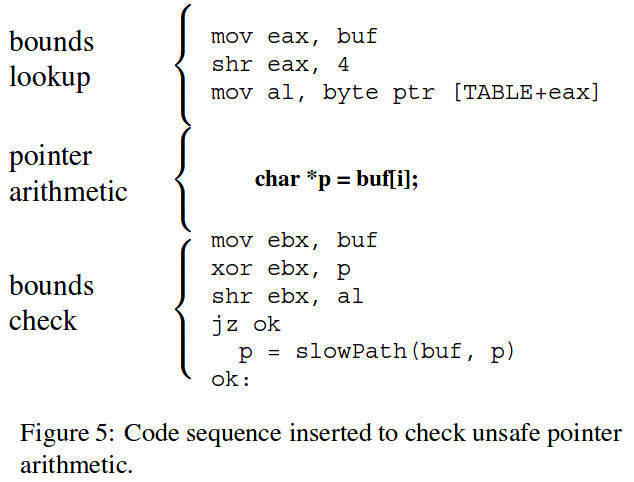
\includegraphics[width=0.6\textwidth]{../bounds/bb-bounds-check}
\end{frame}

\begin{frame}[fragile,label=addedCode]{baggy bounds check: added code}
    \lstset{language=myasm,style=small}
    \begin{lstlisting}
/* bounds lookup */
    mov buf, %rax
    shr %rax, 4
    mov LOOKUP_TABLE(%rax), %al
/* array element address computation */
    ...    // `\textbf{\textit{char * p = buf[i];}}`
/* bound check */
    mov buf, %rbx
    xor p, %rbx
    shr %al, %rbx
    jz  ok
    ...    // handle possible violation
ok:
\end{lstlisting}

    \imagecredit{adapted from paper figure}
\end{frame}

\begin{frame}{avoiding checks}
    \begin{itemize}
        \item code not added if not array/pointer accesses to object
        \item code not added when pointer accesses ``obviously'' safe
            \begin{itemize}
            \item author's implementation: only checked within function
            \end{itemize}
    \end{itemize}
\end{frame}



\subsection{exercise: overhead estimating?}
\begin{frame}<1>[fragile,label=bbOverheadExer1]{exercise: overhead of baggy bounds (1)}
\begin{itemize}
\item suppose program allocates:
    \begin{itemize}
    \item 1000 100 byte objects
    \item 1 10000 byte object
    \end{itemize}
\item using baggy bounds, estimate:
    \begin{itemize}
    \item space required for padding
        \begin{itemize}
        \item<2-> $(128-100)\cdot 1000 + (16384 - 10000)) = 34384$
        \end{itemize}
    \item space required for table
        \begin{itemize}
        \item<2-> $(128\cdot 1000 + 16384) \div 16 = 9024$
        \end{itemize}
    \end{itemize}
\end{itemize}
\end{frame}

\iftoggle{heldback}{}{\againframe<2>{bbOverheadExer1}}

\begin{frame}[fragile,label=bbOverheadExer2]{exercise: overhead of baggy bounds (2)}
\begin{lstlisting}[language=C,style=smaller]
char *strcat(char *d, char *s) {
    int i;
    for (i = 0; s[i] != '\0'; i += 1) {
        d[i] = s[i]; 
    }
    d[i] = '\0';
    return d;
}
\end{lstlisting}
\begin{itemize}
\item estimate:
\begin{itemize}
\item number of bounds checks needed
\item very rough number of instructions run w/o bounds check
\end{itemize}
\item thought question: \\
with bounds checking, what's fastest possible code?
\end{itemize}
\end{frame}


\subsection{alternative: pointer tagging}

\begin{frame}{alternate approach: pointer tagging}
    \begin{itemize}
        \item some bits of \myemph{address} are size 
        \begin{itemize}
        \item replaces table entry/lookup
        \end{itemize}
    \item change code to allocate objects this way
    \item works well on 64-bit --- plenty of addresses to use
    \end{itemize}
    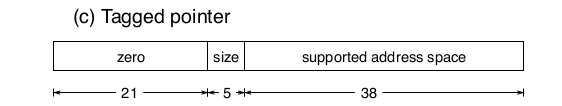
\includegraphics[width=0.8\textwidth]{../bounds/baggy-bounds-tagging}
\end{frame}



\subsection{performance?}

\begin{frame}{baggy bounds performance}
    \begin{itemize}
        \item table: 4--72\% time overhead (depends on benchmark suite)
        \item table: 11--21\% space overhead (depends on benchmark suite)
        \item tagged pointers: slightly better on average
    \end{itemize}
\end{frame}

\begin{frame}{baggy bounds performance}
    \begin{center}
    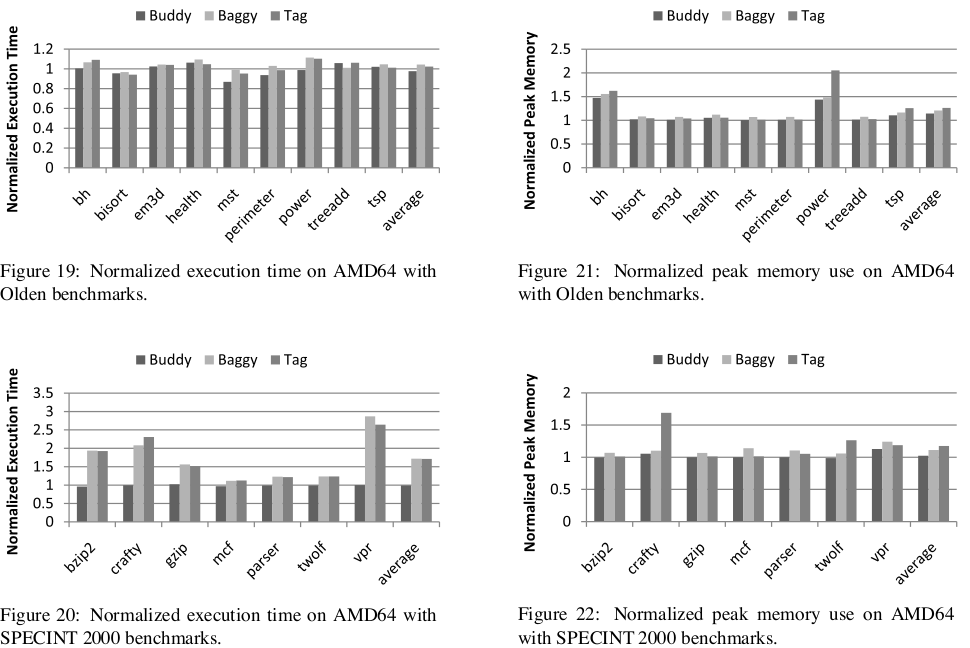
\includegraphics[height=0.8\textheight]{../bounds/baggy-bounds-perf}
    \end{center}
\end{frame}



\subsection{problem: pointers within objects}
% FIXME
\begin{frame}[fragile,label=withinObj]{problem: within object}
\begin{lstlisting}
struct foo {
    char buffer[1024];
    int *pointer;
};
struct foo array_of_foos[1024];
...
char *p = &array_of_foos[4].buffer[4]
\end{lstlisting}
\begin{itemize}
\item exercise: what are the bounds for p?
\end{itemize}
\end{frame}


\subsection{corner cases}

\begin{frame}[fragile,label=unfortunateCProgF2C]{unfortunate things C programmers do (4)}
in code generated by f2c (Fortran to C translator) \\
{\scriptsize (cleaned up slightly)}
\begin{lstlisting}[language=C,style=small]
float sum(int size, float *arr) {
    arr = arr - 1; /* <-- deliberately out-of-bounds pointer */
    float result = 0.f;
    for (i = 1; i <= size; ++i) {
        result += arr[i]
    }
    return result;
}
\end{lstlisting}
\end{frame}



\section{AddressSanitizer}

\begin{frame}{AddressSanitizer}
    \begin{itemize}
    \item like baggy bounds:
        \begin{itemize}
        \item big lookup table
        \item lookup table set by memory allocations
        \item compiler modification: change stack allocations
        \end{itemize}
    \item unlike baggy bounds:
        \begin{itemize}
        \item check reads/writes (instead of pointer computations)
        \item only detect errors that read/write \myemph{between objects}
        \item object sizes not padded to power of two
        \item table has info for every single byte (more precise)
        \end{itemize}
    \end{itemize}
\end{frame}




\subsection{ASan's added check}

\begin{frame}[fragile,label=asanVBounds]{adding bounds-checking example}
\lstset{
    language=C++,
    style=small,
    moredelim={**[is][\btHL<2>]{~2~}{~end~}},
}
\begin{lstlisting}
void vulnerable(long value, int offset) {
    long array[10] = {1,2,3,4,5,6,7,8,9,10};
    // generated code: (added by AddressSanitizer)
    ~2~if (!lookup_table[&array[offset]] == VALID) FAIL();~end~
    array[offset] = value;
    do_something_with(array);
}
\end{lstlisting}
    \begin{itemize}
        \item AddressSanitizer: crashes only if \lstinline|array[offset]| isn't part of any object
            \begin{itemize}
            \item but no extra space --- single-byte precision
            \end{itemize}
    \end{itemize}
\end{frame}



\subsection{stack layout}
\usetikzlibrary{arrows.meta,matrix,patterns}
\tikzset{
    stackBox/.style={very thick},
    allocBox/.style={dashed,very thick,fill=blue!20},
    onStack/.style={thick},
    frameOne/.style={fill=blue!15},
    frameTwo/.style={fill=red!15},
    markLine/.style={blue!50!black},
    markLineB/.style={red!90!black},
    hiLine/.style={red!90!black},
}
\begin{frame}[fragile,label=asanStackLayout]{AddressSanitizer stack layout}
    \begin{tikzpicture}
        \begin{scope}[x=1.7cm]
    \draw[stackBox] (0, 0) rectangle (5, -6);
            \draw[onStack] (0, 0) rectangle (5, -.5)
        node[midway] (arrayLoc) { return address (for \texttt{vulernable()}) };
    \begin{visibleenv}<2>
        \node[anchor=west] at (5.25, -.25) { $\approx$ \tt array[0x13]};
        \node[anchor=west] at (5.25, -3.75) { $\approx$ \tt array[0xa]};
    \end{visibleenv}
    \draw[onStack] (0, -.5) rectangle (5, -1)
        node[midway] { saved \tt\%rbp };
    \draw[onStack] (0, -1) rectangle (5, -1.5)
        node[midway] { saved \tt\%r13 };
    \draw[onStack] (0, -1.5) rectangle (5, -2)
        node[midway] { saved \tt\%r12 };
    \draw[onStack] (0, -2) rectangle (5, -2.5)
        node[midway] { saved \tt\%rbx };
    \draw[onStack,pattern=north west lines,pattern color=red] (0, -2.5) rectangle (5, -4)
        node[midway,fill=white] { ``red zone'' };
    \draw[onStack] (0, -4) rectangle (5, -6)
        node[midway,fill=white] { \tt array };
            \draw[onStack,dashed] (0, -4) rectangle (5, -4.5) node[midway] {\tt array[9]};
            \begin{visibleenv}<3>
            \matrix[tight matrix,
                nodes={text width=3cm,font=\small\tt},anchor=north west,label={north:lookup table}] (tbl) at (6, -2) {
                valid \\ valid  \\ valid \\ valid \\ valid \\ invalid \\ invalid \\
                invalid \\ invalid \\ valid \\ valid \\ \ldots \\
            };
                \draw[thick,-Latex] (5, -.25) -- (tbl-1-1.west);
                \draw[thick,-Latex] (5, -.75) -- (tbl-2-1.west);
            \end{visibleenv}
    \draw[thick,-Latex] (5.15, -6) --++ (0, 2);
        \end{scope}
    \end{tikzpicture}
\end{frame}





\section{AddressSanitizer}

\begin{frame}{AddressSanitizer}
    \begin{itemize}
    \item like baggy bounds:
        \begin{itemize}
        \item big lookup table
        \item lookup table set by memory allocations
        \item compiler modification: change stack allocations
        \end{itemize}
    \item unlike baggy bounds:
        \begin{itemize}
        \item check reads/writes (instead of pointer computations)
        \item only detect errors that read/write \myemph{between objects}
        \item object sizes not padded to power of two
        \item table has info for every single byte (more precise)
        \end{itemize}
    \end{itemize}
\end{frame}




\subsection{ASan's added check}

\begin{frame}[fragile,label=asanVBounds]{adding bounds-checking example}
\lstset{
    language=C++,
    style=small,
    moredelim={**[is][\btHL<2>]{~2~}{~end~}},
}
\begin{lstlisting}
void vulnerable(long value, int offset) {
    long array[10] = {1,2,3,4,5,6,7,8,9,10};
    // generated code: (added by AddressSanitizer)
    ~2~if (!lookup_table[&array[offset]] == VALID) FAIL();~end~
    array[offset] = value;
    do_something_with(array);
}
\end{lstlisting}
    \begin{itemize}
        \item AddressSanitizer: crashes only if \lstinline|array[offset]| isn't part of any object
            \begin{itemize}
            \item but no extra space --- single-byte precision
            \end{itemize}
    \end{itemize}
\end{frame}



\subsection{stack layout}
\usetikzlibrary{arrows.meta,matrix,patterns}
\tikzset{
    stackBox/.style={very thick},
    allocBox/.style={dashed,very thick,fill=blue!20},
    onStack/.style={thick},
    frameOne/.style={fill=blue!15},
    frameTwo/.style={fill=red!15},
    markLine/.style={blue!50!black},
    markLineB/.style={red!90!black},
    hiLine/.style={red!90!black},
}
\begin{frame}[fragile,label=asanStackLayout]{AddressSanitizer stack layout}
    \begin{tikzpicture}
        \begin{scope}[x=1.7cm]
    \draw[stackBox] (0, 0) rectangle (5, -6);
            \draw[onStack] (0, 0) rectangle (5, -.5)
        node[midway] (arrayLoc) { return address (for \texttt{vulernable()}) };
    \begin{visibleenv}<2>
        \node[anchor=west] at (5.25, -.25) { $\approx$ \tt array[0x13]};
        \node[anchor=west] at (5.25, -3.75) { $\approx$ \tt array[0xa]};
    \end{visibleenv}
    \draw[onStack] (0, -.5) rectangle (5, -1)
        node[midway] { saved \tt\%rbp };
    \draw[onStack] (0, -1) rectangle (5, -1.5)
        node[midway] { saved \tt\%r13 };
    \draw[onStack] (0, -1.5) rectangle (5, -2)
        node[midway] { saved \tt\%r12 };
    \draw[onStack] (0, -2) rectangle (5, -2.5)
        node[midway] { saved \tt\%rbx };
    \draw[onStack,pattern=north west lines,pattern color=red] (0, -2.5) rectangle (5, -4)
        node[midway,fill=white] { ``red zone'' };
    \draw[onStack] (0, -4) rectangle (5, -6)
        node[midway,fill=white] { \tt array };
            \draw[onStack,dashed] (0, -4) rectangle (5, -4.5) node[midway] {\tt array[9]};
            \begin{visibleenv}<3>
            \matrix[tight matrix,
                nodes={text width=3cm,font=\small\tt},anchor=north west,label={north:lookup table}] (tbl) at (6, -2) {
                valid \\ valid  \\ valid \\ valid \\ valid \\ invalid \\ invalid \\
                invalid \\ invalid \\ valid \\ valid \\ \ldots \\
            };
                \draw[thick,-Latex] (5, -.25) -- (tbl-1-1.west);
                \draw[thick,-Latex] (5, -.75) -- (tbl-2-1.west);
            \end{visibleenv}
    \draw[thick,-Latex] (5.15, -6) --++ (0, 2);
        \end{scope}
    \end{tikzpicture}
\end{frame}



\subsection{can't change object layout?}
\begin{frame}[fragile,label=withinObj]{revisted: within object}
\begin{lstlisting}
struct foo {
    char buffer[1024];
    int *pointer;
};
struct foo array_of_foos[1024];
...
char *p = &array_of_foos[4].buffer[4]
\end{lstlisting}
\begin{itemize}
\item exercise: What out-of-bounds accesses to `p' can AddressSanitizer detect?
\item how does that compare to baggy bounds? To the `fat pointers' strategy?
\end{itemize}
\end{frame}

\usetikzlibrary{arrows.meta,patterns,shapes.misc}
\tikzset{
    stackBox/.style={very thick},
    allocBox/.style={dashed,very thick,fill=blue!20},
    on stack/.style={thick},
    frameOne/.style={fill=blue!15},
    frameTwo/.style={fill=red!15},
    markLine/.style={blue!50!black},
    markLineB/.style={red!90!black},
    hiLine/.style={red!90!black},
}

\begin{frame}[fragile,label=changeObjLayout]{changing object layout?}
\begin{lstlisting}
struct string_list {
    char data[100];
    struct string_list *prev;
    struct string_list *next;
};
\end{lstlisting}
\begin{tikzpicture}[overlay,remember picture]
\node[anchor=south] at (2.5, 0) {actual layout};
\begin{scope}[shift={(0,0)}]
\draw[on stack] (0, 0) rectangle ++(5, -.5)
    node[midway] {prev};
\draw[on stack] (0, -.5) rectangle ++(5, -.5)
    node[midway] {next};
\draw[on stack] (0, -1) rectangle ++(5, -2)
    node[midway] {data};
\draw[thick,-Latex] (5.25, -3) --++ (0, 1);
\end{scope}
\node[anchor=south] at (9.5, 0) {layout wanted for error-finding};
\begin{scope}[shift={(7,0)}]
\draw[on stack] (0, 0) rectangle ++(5, -.5)
    node[midway] {prev};
\draw[on stack] (0, -.5) rectangle ++(5, -.5)
    node[midway] {next};
\draw[on stack,pattern=north west lines, pattern color=red] (0, -1) rectangle ++(5, -1)
    node[midway] {``red zone''};
\draw[on stack] (0, -2) rectangle ++(5, -2)
    node[midway] {data};
\draw[thick,-Latex] (5.25, -4) --++ (0, 1);
\end{scope}
\begin{visibleenv}<2->
\node[ultra thick,draw,red,cross out,minimum width=5cm,minimum height=4cm] at (9.5, -2) {};
\node[rotate=15,draw,thick,fill=red!10,font=\small,align=center] at (9.5, -3) {
    would break calls to libraries \\
    (unless library also rebuilt)
};
\end{visibleenv}
\end{tikzpicture}
\end{frame}


\subsection{pro/con}

\begin{frame}{AddressSanitizer versus Baggy Bounds}
    \begin{itemize}
    \item pros vs baggy bounds:
        \begin{itemize}
        \item you can actually use it (comes with GCC/Clang)
        \item byte-level precision --- no ``padding'' on objects
        \item detects use-after-free a lot of the time
        \end{itemize}
    \item cons vs baggy bounds:
        \begin{itemize}
        \item doesn't prevent out-of-bounds ``targetted'' accesses
        \item requires extra space between objects
        \item usually slower
        \end{itemize}
    \end{itemize}
\end{frame}



\section{valgrind memcheck, briefly}


\begin{frame}{Valgrind Memcheck}
    \begin{itemize}
    \item similar to AddressSanitizer --- but no compiler modificaitons
    \item instead: is a virtual machine (plus alternate malloc/new implementation)
    \vspace{.5cm}
    \item only (reliably) detects errors on heap
    \item but works on \myemph{unmodified} binaries
    \end{itemize}
\end{frame}




\subsection{aside: binary translation}
% From 20170123
\usetikzlibrary{positioning}

\begin{frame}{binary translation}
    \begin{itemize}
    \item compile assembly to new assembly
    \vspace{1cm}
    \item works without instruction set support
    \item early versions of VMWare on x86 (before x86 added virtualisation support)
    \item can be used to run one platform on another
    \end{itemize}
\end{frame}

\begin{frame}[fragile,label=binTransIdea]{binary translation idea}
\lstset{
    language=myasm,
    style=small,
    morekeywords={movq,addss,subss}
}
\begin{tikzpicture}
\tikzset{
    code/.style={inner sep=0mm,align=left},
    hiOn/.style={alt=#1{rounded corners,fill=green,fill opacity=0.3,text opacity=1.0}{}},
    markOn/.style={alt=#1{rounded corners,draw,thick}{}},
}
\node[code,markOn=<2>,hiOn=<3>] (bb1) {
\begin{lstlisting}
0x40FE00: addq %rax, %rbx
movq 14(%r14,4), %rdx
addss %xmm0, (%rdx)
...
0x40FE3A: jne 0x40F404
\end{lstlisting}
};
\node[right=.25cm of bb1,visible on=<2>,align=left] {
    divide machine code \\
    into \textit{basic blocks} \\
    (= ``straight-line'' code) \\
    (= code till \\ 
    jump/call/etc.)
};
\node[code,right=.25cm of bb1,visible on=<3>] (bb1New) {
generated code: \\
\begin{lstlisting}
// addq %rax, %rbx
movq rax_location, %rdi
movq rbx_location, %rsi
call checked_addq
movq %rax, rax_location
...
// jne 0x40F404
... // get CCs 
je do_jne
movq $0x40FE3F, %rdi
jmp translate_and_run
do_jne:
movq $0x40F404, %rdi
jmp translate_and_run
\end{lstlisting}
};
\node[code,markOn=<2>,anchor=north west] (bb2) at (bb1.south west){
\begin{lstlisting}
subss %xmm0, 4(%rdx)
...
je 0x40F543
\end{lstlisting}
};
\node[code,markOn=<2>,anchor=north west] (bb3) at (bb2.south west){
\begin{lstlisting}
ret
\end{lstlisting}
};
\end{tikzpicture}
\end{frame}

\begin{frame}[fragile,label=binTransIdea2]{a binary translation idea}
    \begin{itemize}
    \item convert whole \textit{basic blocks}
        \begin{itemize}
        \item code upto branch/jump/call
        \end{itemize}
    \item end with call to {\tt translate\_and\_run}
        \begin{itemize}
        \item compute new \myemph{simulated PC} address to pass to call
        \end{itemize}
    \end{itemize}
\end{frame}

\begin{frame}[fragile,label=binTransIdea3]{making binary translation fast}
    \lstset{style=small,language=myasm,morekeywords={movq}}
    \begin{itemize}
    \item cache converted code
        \begin{itemize}
        \item {\tt translate\_and\_run} checks cache first
        \end{itemize}
    \item patch calls to {\tt translate\_and\_run} to refer directly to cached code
    \item do something more clever than \lstinline|movq rax_location, ...|
        \begin{itemize}
        \item map (some) registers to registers, not memory
        \end{itemize}
    \item ends up being ``just-in-time'' compiler
    \end{itemize}
\end{frame}


\begin{frame}{binary translation? really?}
    \begin{itemize}
    \item early VMWare: for instructions without hardware virtualization support
        \begin{itemize}
        \item only needed for little bits of OS code
        \end{itemize}
    \item used by Apple to handle changing CPU designs
    \item Rosetta 2: run Intel on ARM (current)
    \item Rosetta: run Power PC on Intel (2005--2011)
    \item Mac 68k emulator: Run Motorola 680x0 on Power PC (1994--2005)
    \end{itemize}
\end{frame}



\subsection{aside: other binary translation applications}
% FIXME

\section{exericse: which prevents}
\begin{frame}{which scheme prevents\ldots?}
\begin{itemize}
\item which schemes detect or prevent from being harmful\ldots?
    \begin{itemize}
    \item 1. call to assembly code that goes beyond buffer?
    \item 2. allowing attacker to insert 150 bytes in 100 byte buffer on heap?
    \item 3. allowing attacker to insert 120 bytes in 100 byte buffer on stack?
    \item 4. attecker exploiting code that does array[attacker\_index] to overwrite something outside heap array?
    \end{itemize}
\item of:
    \begin{itemize}
    \item A. ``fat pointers'' approach
    \item B. Baggy Bounds checking
    \item C. AddressSanitizer
    \item D. Valgrind Memcheck
    \end{itemize}
\end{itemize}
\end{frame}

\begin{frame}{answer (1)}
\begin{itemize}
\item which schemes detect or prevent from being harmful\ldots?
    \begin{itemize}
    \item 1. call to assembly code that goes beyond buffer?
    \end{itemize}
\item only Valgrind Memcheck handles assembly code
\item other techniques require C compiler to produce different assembly
\end{itemize}
\end{frame}

\begin{frame}{answer (2)}
\begin{itemize}
\item which schemes detect or prevent from being harmful\ldots?
    \begin{itemize}
    \item 2. allowing attacker to insert 150 bytes in 100 byte buffer on heap?
    \end{itemize}
\item schemes:
    \begin{itemize}
    \item A. ``fat pointers'' approach --- yes
    \item B. Baggy Bounds checking ---yes, detect + crash
    \item C. AddressSanitizer --- yes, detect + crash
    \item D. Valgrind Memcheck --- yes, detect + rash
    \end{itemize}
\end{itemize}
\end{frame}

\begin{frame}{answer (3)}
\begin{itemize}
\item which schemes detect or prevent from being harmful\ldots?
    \begin{itemize}
    \item 3. allowing attacker to insert 120 bytes in 100 byte buffer on stack?
    \end{itemize}
\item schemes:
    \begin{itemize}
    \item A. ``fat pointers'' approach --- yes
    \item B. Baggy Bounds checking ---prevent from being harmful / no crash
    \item C. AddressSanitizer --- yes, detect + crash (red zone)
    \item D. Valgrind Memcheck --- no --- no memory to mark invalid
    \end{itemize}
\end{itemize}
\end{frame}

\begin{frame}{answer (3)}
\begin{itemize}
\item which schemes detect or prevent from being harmful\ldots?
    \begin{itemize}
    \item 4. attecker exploiting code that does array[attacker\_index] to overwrite something outside heap array?
    \end{itemize}
\item schemes:
    \begin{itemize}
    \item A. ``fat pointers'' approach --- yes
    \item B. Baggy Bounds checking --- yes
    \item C. AddressSanitizer --- no --- attacher index can find valid memory
    \item D. Valgrind Memcheck --- no --- (same as AddressSanitizer)
    \end{itemize}
\end{itemize}
\end{frame}

% FIXME: exercise
    % which scheme will prevent XXX



\section{backup slides}
\begin{frame}{backup slides}
\end{frame}



%\iftoggle{heldback}{}{
%\subsection{narayan slides}
%\includepdf[pages=13-24]{../sandbox/sec20_slides_narayan.pdf}
%}


\end{document}
